%%%%%%%%%%%%%%%%%%%%%%%%%%%%%%%%%%%%%%%%%%%%%%%%%%%%%%%%%%%%%%%%%%%%%%%%%%%%%%%%%%%%%%%%%%%%%%%%%%%%%%%%%%%%%%%%%%%%%%%%%%%%%%%%%%%%%%%%%%%%%%%%%%%%%%%%%%%
% This is just an example/guide for you to refer to when submitting manuscripts to Frontiers, it is not mandatory to use Frontiers .cls files nor frontiers.tex  %
% This will only generate the Manuscript, the final article will be typeset by Frontiers after acceptance.   
%                                              %
%                                                                                                                                                         %
% When submitting your files, remember to upload this *tex file, the pdf generated with it, the *bib file (if bibliography is not within the *tex) and all the figures.
%%%%%%%%%%%%%%%%%%%%%%%%%%%%%%%%%%%%%%%%%%%%%%%%%%%%%%%%%%%%%%%%%%%%%%%%%%%%%%%%%%%%%%%%%%%%%%%%%%%%%%%%%%%%%%%%%%%%%%%%%%%%%%%%%%%%%%%%%%%%%%%%%%%%%%%%%%%

%%% Version 3.4 Generated 2018/06/15 %%%
%%% You will need to have the following packages installed: datetime, fmtcount, etoolbox, fcprefix, which are normally inlcuded in WinEdt. %%%
%%% In http://www.ctan.org/ you can find the packages and how to install them, if necessary. %%%
%%%  NB logo1.jpg is required in the path in order to correctly compile front page header %%%

\documentclass[utf8]{frontiersSCNS} % for Science, Engineering and Humanities and Social Sciences articles

%\setcitestyle{square} % for Physics and Applied Mathematics and Statistics articles
\usepackage{url,hyperref,lineno,microtype,subcaption}
\usepackage[onehalfspacing]{setspace}
\linenumbers
% Leave a blank line between paragraphs instead of using \\

\def\keyFont{\fontsize{8}{11}\helveticabold }
\def\firstAuthorLast{El Damaty {et~al.}} %use et al only if is more than 1 author
\def\Authors{Shady El Damaty\,$^{1,2*}$, Veronica Mucciarone\,$^{2}$, Yewon Chun, Marissa L. Laws$^{1}$, Victor Campano, Diana H. Fishbein\,$^{3}$ and John W. VanMeter\,$^{1}$}
% Affiliations should be keyed to the author's name with superscript numbers and be listed as follows: Laboratory, Institute, Department, Organization, City, State abbreviation (USA, Canada, Australia), and Country (without detailed address information such as city zip codes or street names).
% If one of the authors has a change of address, list the new address below the correspondence details using a superscript symbol and use the same symbol to indicate the author in the author list.
\def\Address{$^{1}$Interdisciplinary Program in Neuroscience, Georgetown University, Washington, District of Columbia, USA 
$^{2}$Center for Functional \& Molecular Imaging, Georgetown University Medical Center, Department of Neurology, Washington, District of Columbia, USA
$^{3}$ }

% Laboratory X, Institute X, Department X, Organization X, City X , State XX (only USA, Canada and Australia), Country X 
% The Corresponding Author should be marked with an asterisk
% Provide the exact contact address (this time including street name and city zip code) and email of the corresponding author
\def\corrAuthor{Shady El Damaty}
\def\corrEmail{se394@georgetown.edu}
\begin{document}
\onecolumn
\firstpage{1}
\title{Introducing an Adolescent Neurocognitive Maturity Index Derived from Behavioral Task Performance Metrics} 
\author[\firstAuthorLast ]{\Authors} %This field will be automatically populated
\address{} %This field will be automatically populated
\correspondance{} %This field will be automatically populated
\extraAuth{}
%\extraAuth{corresponding Author2 \\ Laboratory X2, Institute X2, Department X2, Organization X2, Street X2, City X2 , State XX2 (only USA, Canada and Australia), Zip Code2, X2 Country X2, email2@uni2.edu}
\maketitle \begin{abstract}
%%% Leave the Abstract empty if your article does not require one, please see the Summary Table for full details.
\section{}
% For full guidelines regarding your manuscript please refer to \href{http://www.frontiersin.org/about/AuthorGuidelines}{Author Guidelines}.
% As a primary goal, the abstract should render the general significance and conceptual advance of the work clearly accessible to a broad readership. References should not be cited in the abstract. Leave the Abstract empty if your article does not require one, please see \href{http://www.frontiersin.org/about/AuthorGuidelines#SummaryTable}{Summary Table} for details according to article type. 

\tiny
 \keyFont{ \section{Keywords:} adolescence, cognitive development, age prediction, maturity, dual systems model} %All article types: you may provide up to 8 keywords; at least 5 are mandatory.
\end{abstract}
%%%%%%%%%%%%%%%%%%%%%%%%%%%%%%%%%%%%%%%%%%%%%%%%%%%%%%%%%%%%%%%%%%%
\section{Introduction}
%%%%%%%%%%%%%%%%%%%%%%%%%%%%%%%%%%%%%%%%%%%%%%%%%%%%%%%%%%%%%%%%%%%
The transition from adolescence to young adulthood is marked by the maturation of core cognitive control skills required for adaptive social decision-making in the execution of goal-directed behavior. These skills include active maintenance of goal-related representations in working memory, task switching, inhibitory control of reflexive behavior, weighting of risks versus rewards, and processing emotional context \citep{luna2015integrative}. Cognitive skill development during adolescence co-occurs with increased sensitivity to reinforcement signals in the form of positive or negative outcomes during social and generic task learning. Supporting this view are several complementary models of adolescent brain development describing adolescence as a period of mismatch between the efficiency of cognitive control and salience of perceived rewards \citep{Steinberg2010, CaseyEtAl2008, LunaWright2016, rosenbaum2020valence}. These models are corroborated by both behavioral and non-invasive neuroimaging evidence, suggesting that cognitive skills and brain regions associated with these skills indeed develop during adolescence.  However, the exact timing of cognitive skill maturation and the interaction between cognitive control, risk taking, and emotion processing is not yet fully understood \citep{shulman2016dual, duell2016interaction}.\paragraph*{} Several lines of research on biomarkers of age-related change have demonstrated maturation is a complex transformational event affected by both biological and environmental mechanisms that can vary significantly across individuals. Social adversity in particular has been shown to accelerate sexual maturation \citep{rickard2014childhood}, drive puberty-related epigenetic moderators of depressive symptoms \citep{sumner2019early}, impair developmental decreases in brain gray matter volume, and corresponding increases in white matter integrity \citep{gur2019burden, Gogtay2004}; as well as alter development of both functional brain network topology \citep{tooley2020associations} and cognitive skills \citep{mclaughlin2019childhood, belsky2019early}. \paragraph*{} The maturational timing of risk/reward processing and inhibitory control skills is hypothesized to uniquely interact with the social pressures associated with achieving independence in early adulthood. Disruptions to a normative maturational trajectory may consequently lead to poor adjustment, anti-social attitudes, and the increased likelihood of adverse outcomes. Epidemiological data clearly illustrate  that growing up, in-of-itself, is the greatest risk factor for a non-health related adverse outcome throughout all of lifespan development \citep{turner2006effect}. In 2008, approximately 60\% of youth under the age of 17 had experienced assault, sexual abuse, childhood maltreatment or either dating, domestic or community violence \citep{finkelhor2009children}.  These statistics suggest that the transitional period to adulthood is a key point of vulnerability during lifespan development \citep*{berzin2010vulnerability}. \paragraph*{} Although existing models of adolescent cognitive development have been helpful for understanding the transition to adulthood, a key missing aspect is a data-driven [operationalized] definition of neurocognitive age, or maturity. A precise definition has potential to fill existing knowledge gaps and help translate science for utilitarian social applications  \citep{somerville2016searching}. Early biological models of age based on DNA methylation, transcription and telomere length \citep{baker1988biomarkers, jylhava2017biological}, brain structure \citep{khundrakpam2015prediction,aycheh2018biological,madan2018predicting}, and brain network oxygen metabolism \citep{dosenbach2010prediction, qin2015predicting} have exhibited significant success for predicting age and identifying sample-relative individual developmental trajectories. However, neurocognitive age prediction has yet to be implemented with theory-driven indicator variables obtained from behavioral experiments. \paragraph*{} The absence of a complete theoretical model of biological mechanisms underlying age-related changes has led to a proliferation of analytic techniques using a substantial number of features to extrapolate sample-specific effects. Common methods for age prediction are typically big-data-driven, involving the collection of large amounts of data per individual, such as genome-wide RNA transcription, or MRI measurements analyzed using hundreds of thousands of pair-wise correlations between voxels at discrete time intervals. These methods pose an issue in that there are significantly more descriptive features per individual than there are samples in the dataset (i.e., $p >> n$), a problem that commonly leads to overfitting with standard linear regression. This problem is overcome through the application of data reduction and variable selection techniques such as principal component analysis or regularized regression that penalizes or eliminates redundant features. These model-free techniques have been successful in predicting age within an acceptable error range \citep{cole2017predicting}. However, they do not always lend themselves to interpretation because variable selection and data reduction can be biased by their cost function, leading to overfitting \citep{babyak2004you}, or confounded by correlates of age, such as motion in fMRI experiments \citep{satterthwaite2013heterogeneous}. \paragraph*{} A potential solution may be to use data collected from theory-driven experimental designs that identify and measure specific features of age-related change for model fitting. Currently, there are no applications utilizing well-validated behavioral tasks for testing dual-systems type models with the goal of estimating neurocognitive age in typically developing adolescents. Here, we describe a simple method for computing a neurocognitive maturity index (NCMI) derived from reaction time, task performance, and and related metrics from the Continuous Performance (CPT), Wheel of Fortune (WOF), and Emotional Face Recognition (EFR) tasks collected in the Adolescent Development Study \citep{Fishbein2016}. Using Confirmatory Factor Analysis, we estimate latent factors for inhibitory control, risk/reward processing, and sensitivity to emotion. Latent factor analysis composes a first-pass, theory-driven data reduction technique which estimates directly unobservable mechanisms expected to change with age. The interaction between factors is tested in a structural equation model (SEM) and latent factor estimates are used as predictors in a regularized regression model to predict age. The NCMI is thus defined as the difference between observed and predicted cognitive age. A high NCMI indicates accelerated cognitive maturity relative to the sample mean, whereas a low NCMI indicates a relatively lagging developmental trajectory. In this sample, high NCMI predicted elevated risk for future violent outcomes, which was mediated by behavioral drive for achieving independence. This work demonstrates that predicting cognitive age using latent constructs is a promising pursuit which can be scaled with larger neurocognitive datasets. This method may facilitate generation of population estimates for adolescent neurocognitive maturity which may be used to explore predictive models of adverse outcomes and further illuminate the interaction between social context and trajectories of neurocognitive development. 
%%%%%%%%%%%%%%%%%%%%%%%%%%%%%%%%%%%%%%%%%%%%%%%%%%%%%%%%%%%%%%%%%%%
\section{MATERIALS AND METHODS}
%%%%%%%%%%%%%%%%%%%%%%%%%%%%%%%%%%%%%%%%%%%%%%%%%%%%%%%%%%%%%%%%%%%
\subsection{Participants} Volunteers were recruited from the Adolescent Development Study (ADS), a prospective, longitudinal investigation of the neurodevelopmental factors underlying early substance use initiation \citep{Fishbein2016}. Youth from the Washington, D.C. Metro area were first enrolled in 2011 ($53.6\%$ female; $52\%$ Caucasian, $32.8\%$ African-American, $6.7\%$ Hispanic and/or Latino, $8.2\%$ Other) and, as of March 2020, have completed four waves of data collection separated by approximately 18 months. Eligibility at wave 1 included the following criteria: 1) ages 11-13 years, 2) right-handedness, 3) no history of neuropsychiatric disorders or recent head injuries, 4) no self-reported use of drugs or alcohol and 5) no direct Asian descent. A total of six participants were excluded following the baseline visit due to: substance use at baseline ($N=2$), autism diagnosis ($N=1$), and high scores on ambidexterity measured with the Edinburgh Handedness Test ($N=3$) \citep{veale2014edinburgh}. Study visits during the first three waves (wave $1$: $N=140$, ages $11.1$ - $14.0$ years; wave $2$:  $N=123$, ages $12.4$ - $16.1$ years; wave $3$: $N=113$, ages $13.9 - 18.0$ years) were comprised of sociodemographic interviews with the parent and child, ascertaining child self-reported drug use via automated questionnaires, as well as neuropsychological testing of risk-taking, inhibitory control and emotional face processing. Despite attrition, the distribution of sex and race remained approximately the same throughout the study (+/- $0.5\%$) . The fourth wave ($N=74$, ages $14.80$ - $20.65$ years; mean $18.76$ years, $54.1\%$ female, $60.3\%$ Caucasian, $28.8\%$ African-American, $4.2\%$ Hispanic and/or Latino, $6.8\%$ Other) was conducted as an extension funded by the National Institute of Justice aimed at following up on violent outcomes in adulthood \citep{ElDamaty2016NIJ}. Participants were recontacted for follow up with in-person or through online surveys in the case of those that had relocated a significant distance from the study site. Sociodemographic measures were selected from The Centers for Disease Control and Prevention’s Violence Prevention Compendium to measure experiences of violence in adulthood \citep{dahlberg2005measuring}. Participants were compensated \$$60$ and reimbursed for travel, when applicable. All youth and caregivers gave their informed assent and consent prior to data collection and study procedures were reviewed and approved by the Georgetown University Institutional Review Board.
%%%%%%%%%%%%%%%%%%%%%
% Interview
%%%%%%%%%%%%%%%%%%%%%
\subsection{Interview Procedure and Collected Metrics} Pre-screened, eligible participants were invited for an on-site visit at Georgetown University Medical Center to complete a series of questionnaires and interviews designed to measure neurocognitive developmental traits and capture social and family life. Parents and/or primary guardians accompanied participants that were minors and family members were interviewed in separate rooms. The guardian and/or parent was asked to complete a questionnaire regarding economic status, education and information regarding the difficulty of acquiring basic needs such as food, healthcare and housing \citep{bornstein2003socioeconomic}. Socioeconomic Status (SES) was estimated from these responses by converting the family’s household income to z-scores, averaging both guardian/parents' years of education, converting the average to a z-score, and lastly averaging the income and education z-scores for the final SES measure (method adapted from \cite{manuck2010ses}).
%%%%%%%%%%%%%%%%%%%%%
% Anthropometrics
%%%%%%%%%%%%%%%%%%%%%
\paragraph{Anthropometrics} At each timepoint, adolescents had their height and weight measured and completed a pubertal scale survey \citep{carskadon1993self} to measure physical changes with age.  Pubertal development scores were derived from from reported changes in height, body hair, complexion, vocal pitch, breast size, and menstruation. Respondents would indicate “has not yet begun,” “has barely begun,” “is definitely underway,” or “is complete” for each puberty related physical feature queried by the instrument. Responses were numerically coded and normalized relative to the sample mean.
%%%%%%%%%%%%%%%%%%%%%
% Instruments
%%%%%%%%%%%%%%%%%%%%%
\paragraph{Instruments} Risk for future adverse outcomes (i.e., substance abuse, mood disorders, delinquent behavior) and future violence proneness was measured with the revised Drug Use Screening Inventory (DUSI-R) in waves $1$ through $3$ \citep{tarter1994reliability}. The DUSI-R is composed of 10 subscales: substance abuse, behavioral problems, psychiatric disturbances, medical problems, family dysfunction, work problems, school maladjustment, social skills deficiency, peer relationship problems, and maladaptive leisure and recreation activities. The average score across scales is indicative of the probability of developing a substance use disorder by age 18. In the present study, the DUSI-R is used to compute a metric for Violence Proneness - an estimation of the risk of experiencing violence in adulthood, either as a victim or perpetrator \citep{kirisci2009violence}. The Violence Proneness metric reflects the average of the school ($7$ items) and peer relations problems ($6$ items) subscales. All youth participants were also assessed for verbal and performance IQ using the Kaufman Brief Intelligence Test (KBIT), \citep{kaufman2004kaufman}. Finally, adolescents completed The Behavioral Inhibition System/Behavioral Activation System (BIS/BAS) Scale  to provide a measure of appetitive and avoidant behavioral tendencies \citep{carver1994behavioral}. The BAS is further divided into three subscales measuring funseeking (BAS-FS), independent drive (BAS-D) and reward responsivity (BAS-RR).
%%%%%%%%%%%%%%%%%%%%%
% Violence Experience
%%%%%%%%%%%%%%%%%%%%%
\paragraph{The Experience of Violence in Adulthood} At the fourth follow-up time point, participants completed a custom-developed instrument designed to capture holistic components of violence experience including general perceptions, direct observations, victimization, and perpetration of violent acts at home, at school or in the community within the last $12$ months. Participants were also asked to specify whether they had heard of, seen or been a victim of violence perpetrated by a civil authority figure, such as a police officer or teacher. The survey contains ranked choice responses (Never = $0$, Once = $1$, Sometimes ($3$-$5$ times) = $2$ and Often ($5+$ times) = $3$) numerically coded and normalized by summing across the responses and dividing by the total number of within-scale items to generate a value between $0$ and $1$. The instrument provides the following subscales: perception of violence ($5$ items), observation of violence ($5$ items), violent victimization ($5$ items) and perpetration of violence ($7$ items). The observation, perception and victimization subscales may be divided into an additional measure of violence relating to civil authority figures. Confirmatory latent factor analysis utilizing these derived subscales was used to validate and estimate a subject-specific latent factor estimate of holistic violence experience in adulthood ($RMSEA = 0.04$, $p = 0.363$, $CLI = 0.989$).
%%%%%%%%%%%%%%%%%%%%%
% Neurocognitive Tasks
%%%%%%%%%%%%%%%%%%%%%
\subsection{Neurocognitive Tasks}  Participants completed the Continuous Performance (CPT) and Wheel of Fortune (WOF) tasks while undergoing functional MRI (Siemens Tim Trio 3T Scanner) during waves 1-3. Stimuli were projected onto a screen and reflected into the participant's field of view using a mirror. The head was fixed with foam pads and participants were advised to minimize their motion to maintain high quality images. The Emotional Face Recognition (EFR) and Temporal Discounting tasks were completed outside of the scanner on a laptop in a private behavioral testing room. The Facial Emotion Recognition Task was administered with E-Prime 1.2. All other neurocognitive tasks were built and presented with the E-prime Stimulus Presentation Software Version 2.0\citep{schneider2002prime}. 
%%%%%%%%%%%%%%%%%%%%%
% WOF
%%%%%%%%%%%%%%%%%%%%%
\paragraph{Wheel of Fortune Task (WOF)} A modified version of the Wheel of Fortune (WOF) task was administered to test propensity of risk-taking and gambling strategies \citep{ernst2004wheeloffortune}. The task was divided into three runs of 30 trials. In each trial, a "wheel" appeared on the screen that portrayed the probabilities of winning different amounts of virtual money. Participants were instructed to select between either a low chance of winning a large amount (high-risk) or a high chance of winning a small amount (low-risk) and indicated their choice using fiber optical response button boxes placed in the left and right hands (corresponding to choice of the left and right of the wheel, respectively). Winning probability varied pseudo-randomly between a $10:90\%$ split (occurring $32$ to $42$ times of a total $90$ trials) and a $30:70\%$ split (occurring $48$ to $58$ times). The quantitites of money assigned to the left and right side of the wheel varied between a \$$1$ - \$$9$ for the low risk choice or a \$$2$ - \$$18$ split for the high risk choice, when the wheel was split $10:90$ low-risk/high-risk. The quantities similarly varied between \$$3$ - \$$7$ or a \$$9$ - \$$21$ split when the wheel was divided $30:70$.  These values and proportional assignments assured that the expected value (EV) appeared equal for a winning selection independent of risk (e.g., $30\%$ chance of winning \$$7 = $\$$2.10$ EV vs. $70\%$ chance of winning \$$3 =$ \$$2.10$ EV).  Spatial position of the rewards varied evenly, with the larger reward appearing on each side $50\%$ of the time.  The wheel was presented until the participant made their selection, or for a maximum of $3000$ms, followed by a $3000$ms delay. Feedback was presented for $3000$ms after the delay, indicating whether the participant had won or lost the selected dollar amount, along with their running cumulative winnings for that run.  Participants automatically lost the higher dollar amount if no decision was made before $3000$ms had elapsed.  Each run began with a $6000$ms fixation, and inter-trial fixations were varied based on a Poisson distribution between $2500$ to $10000$ms. The total quantity of money won or lost would be reset to \$$0$ at the beginning of each run. Participants were encouraged to improve their strategy for the next run.  All participants were explicitly told that no real money or physical reward would be given. Task performance was analyzed using the probability of high vs. low risk decisions, the reaction time to make those decisions and the cumulative winnings at each run. Anticipatory responses were defined as trials $<200$ms reaction time and discarded from analysis as outliers.
%%%%%%%%%%%%%%%%%%%%%
% CPT
%%%%%%%%%%%%%%%%%%%%%
\paragraph{Continuous Performance Task (CPT)} The continuous performance task was completed by participants to measure impulsivity and inhibitory control of reflexive actions \citep{horn2003response}.  Participants viewed five blocks of $30$ letters presented one-at-a-time for a $200$ms duration (150 total trials). Each block was separated by a "cool-down" period in which a gray fixation cross was presented for a $1300$ms interval. Participants were instructed to press the right-hand button box as quickly as possible for all letters except “Q”. The lure "Q" appeared 27 times in the task. The sequence of letters was the same across all participants.  Signal Detection Theory metrics were utilized for analyzing CPT behavior \cite{stanislaw1999calculation}. Hits were defined as correct button presses to target letters and Misses as missed opportunities to respond to a target letter. False-Alarms were defined as an incorrect response to the the lure "Q" whereas Correct Rejections were defined as correct inhibition of response. Discriminative sensitivity to lures was measured by the $d'$ variable, $d'=\phi^{-1}( Hits ) - \phi^{-1}( False Alarms )$ and response-bias utilizing the natural log-transformed beta estimate, $ \beta = 0.5*\Big[\phi^{-1}(FalseAlarms)^{2} - \phi^{-1}(Hits)^{2}\Big]$. 
%%%%%%%%%%%%%%%%%%%%%
% WOF
%%%%%%%%%%%%%%%%%%%%%
\paragraph{Emotional Face Recognition Task (EFR)} Participants viewed $70$ photographs (grayscale images, $284$ x $351$ pixels, resolution = $96$ dpi) of twenty-nine professional actors ages $21$-$30$ ($12$ female, $17$ male, $14$ European-American, $10$ African-American, $3$ Asian-American $2$ Latino-American) instructed to pose for expressions of $7$ emotions: happiness, surprise, sadness, anger, disgust, fear and neutral \citep{tottenham2009nimstim}. To prepare for the task, participants were presented showcards with labels of each of $7$ emotions and asked to describe/demonstrate each of the emotions followed by a practice trial for each emotion. For each trial, a photograph appeared for a maximum duration of $5000$ms along with $7$ labels for each of the emotions. Participants were instructed to click on the emotion with a mouse to advance to the next trial. The image disappeared after $5000$ms and labels remained until a response was made. An inter-trial interval of $3000$ms of white screen separated each trial. No actor-emotion combination was repeated more than once. The accuracy and reaction time for disgust, anger, sadness and fear were averaged together to compose estimates of performance for recognizing negative emotion. Performance on positive emotion recognition was measured with happiness reaction time and accuracy to happy faces. 
%%%%%%%%%%%%%%%%%%%%%
% TD
%%%%%%%%%%%%%%%%%%%%%
\paragraph{Temporal Discounting Task (TDT)} Individual preference between small and immediate vs. large but delayed rewards was tested by offering participants a forced choice between two options: "Would you rather have \$$X$ now or \$$X+Y$ in $Z$ days?" The delay of rewards $Z$ was varied from zero, one, two, ten days, 1 month, half a year and one year. The presented immediately available amount was determined using a random adjustment procedure that updated the current choice based on previous choices. Immediate reward amounts varied from \$$0.50$ to \$$10$ while the delayed reward value was fixed at \$$10$. The propensity for discounting the objective value due to delayed receipt was computed as the area under the curve (AUC) using the trapezoidal method: $AUC = \sum_{t=0}^{t=k} (d_{t+1}-d_t)*(v_t+v_{t+1} /2)$, where $t$ is the current normalized delay point, $k$ the maximum delay and $v$ the indifference value at that point \citep{Borges2016,olson2007adolescents, myerson2001area}. Indifference points reflecting the subjective value of the immediately available reward at a given delay were normalized to the maximum award value \$$10$ and plotted across annualized time delays. As described above, trapezoids formed by normalized subjective values at each normalized delay contributed to AUC, ranging from 0 - 1.  A large AUC indicates participants are more likely to prefer large but delayed rewards whereas a lower AUC indicates preference for immediate gratification. In order to elicit behavior reflective of the participant's actual preferences, prior to the task, participants were informed that they would receive either a \$$5$ or \$$10$ reward based randomly on their choices in the task. Participants would be more likely to receive a \$$5$ payout immediately after the visit concluded if they selected small and quick rewards more frequently than large, but delayed rewards. Otherwise, their reward was more likely to be a \$$10$ check mailed to the participant 30 days after the visit. 
%%%%%%%%%%%%%%%%%%%%%
% Analysis Methods
%%%%%%%%%%%%%%%%%%%%%
\subsection{Statistical Analysis} Data was converted from double-entered paper records, Qualtrics survey exports, and E-prime task outputs then consolidated into a single long-format data frame containing an observation for each participant at each wave. Descriptive statistics and assessments of multivariate normality were performed with the Arsenal (3.5.0), MVN (5.8, \cite{MVN}) and DescTools (0.99.36, \cite{DescTools}) R packages in R version Orange Blossom (1.2.5033, \cite{R}). Neuropsychological, social and environmental measures were correlated with age to identify and confirm expected bivarate relationships with development. Confirmatory Factor Analysis for identifying latent factors underlying inhibitory control, risk/reward processing and emotional face recognition was completed with the Lavaan package version 0.6-6 \citep{Lavaan}. Participants with high DUSI LIE scores ($>6$) were excluded from analysis \cite{dalla2003effects}. High LIE scores significantly covaried with elevated response bias (Pearson's $R=0.24$) on the CPT and exhibited spurious responses across instruments (such as faster than average completion with very low average reaction times and/or minimal variance in choices with repetitive all "no"/"false" choices). High LIE score was also found to significantly correlate with lower SES ($R=0.25$), important source of potential bias on statistical inference.  Maximum likelihood estimation with full information maximum likelihood (FIML) was used to adjust parameter estimates for missing data \citep{cham2017full}. Latent factors were standardized to allow for free estimation of factor loadings \citep{HuTzeBentler1998}. Goodness of Fit of estimated latent factor models and their structural relations was assessed using the Root Mean Square Error of Approximation (RMSEA), the Comparative Fit Index (CFI) and the Tucker-Lewis Index (TLI \cite{KennyEtAl2015,HuTzeBentler1999}). Structural Equation Path models were visualized with the semPlot package (1.1.2). Age prediction was carried out with regularized linear regression models implemented in the glmnet package (4.0-2) using leave-one-out cross-validation for estimation of model hyperparameters and a 50\% split between training and test datasets \citep{FriedmanHastieTibshirani2010, friedman2009glmnet}. Cross-validated model performance was estimated by computing the $R^2$ from the mean cross-validated error divided by the variance of observed age in the test sample across $\lambda$ and $\alpha$ hyper-parameter estimates. The minimum lambda at the highest $R^2$ was used to calculate regression coefficients in the training sample. The neurocognitive maturity index was estimated as the difference in the observed and predicted age for each participant. Coefficients for mediation and path analysis of relations between NCMI, indicator variables and outcomes were estimated using the lavaan structural equation framework.
%%%%%%%%%%%%%%%%%%%%%%%%%%%%%%%%%%%%%%%%%%%%%%%%%%%%%%%%%%%%%%%%%%%%%%%%%%%%%%%%%%%%
\section{Results} 
%%%%%%%%%%%%%%%%%%%%%%%%%%%%%%%%%%%%%%%%%%%%%%%%%%%%%%%%%%%%%%%%%%%%%%%%%%%%%%%%%%%%
% Latent Factor Analysis
\subsection{Latent Factor Analysis of Cognitive Metrics} 
%%%%%%%%%%%%%%%%%%%%%
% Inhibitory Control
%%%%%%%%%%%%%%%%%%%%%
\paragraph{Inhibitory Control} Inhibitory control was characterized by consistently careful responses and greater discrimination between targets and false alarms in the CPT along with overall idiosyncratic behavioral inhibition. The inhibitory control latent factor (ICLF) was estimated using the CPT response time standard deviation, response bias ($ln(\beta$)), target discrimination ($d'$), and BIS. Response time standard deviation was selected for the model \textit{a priori} because mean reaction time did not significantly vary trial-by-trial across participants except at the beginning of a block (Figure \ref{fig:1}). Additionally, participants were instructed to press the response button as fast as possible and variations in responses were typically only observed circa false alarm trials during which more cautious participants would modify their pace to avoid errors. Task performance increased from wave 1 to 3 (Figure \ref{fig:2}). The fitted relations were significant compared to a null model with 0 factor loadings between all measures, residual covariances, and the latent variable estimate ($CLI = 1.0$, $TLI = 1.017$, $RMSEA << 0.01$; $p = 0.91$). ICLF was characterized by greater target discrimination (standardized estimate $0.649\pm0.090$; $Z = 7.188$; $p<0.001$), lower response bias ($-0.503\pm0.134$; $Z=-4.054$; $p<0.001$), higher behavioral inhibition ($0.193\pm0.058$; $Z=3.327$; $p=0.001$) and generally less variable response times to both targets ($-0.912\pm0.115$; $Z=-7.920$; $p<0.001$) and false-alarms ($-0.372\pm0.085$; $Z=-4.383$). Greater discriminative ability between false alarms and targets was significantly inversely correlated to response bias ($-0.464\pm0.138$; $Z=3.364$; $p=0.001$, Figure \ref{fig:3}) and covaried with greater variation in response time to targets ($0.302\pm0.090$; $Z=3.356$; $p=0.001$), suggesting participants modified their behavior and responded with more consistent timing as they learned the task. This was corroborated by a strong linear relationship between $d'$ and the average response time to targets (estimated linear model coefficient $0.5705\pm0.05$; $Z=12.11$; $p<0.001$). Response time error to targets interacted inversely with false alarm response time to predict $d'$ ($-0.0818\pm0.02$;  $Z=-3.346$; $p < 0.001$) indicating that early false alarms led to greater caution, resulting in overall target/lure discrimination and improved CPT performance. Response time variation was uncorrelated between target and false alarm trials ($0.066\pm0.094$; $Z=0.703$; $p=0.482$) demonstrating that each provided a statistically independent contribution to ICLF. The ICLF did not vary by sex but was found to significantly covary with socioeconomic status (estimated regression coefficient $0.267\pm0.053$; $Z=4.99$; $p<0.001$). 
%%%%%%%%%%%%%%%%%%%%%
% Risk/Reward
%%%%%%%%%%%%%%%%%%%%%
\paragraph{Risk Taking} The risk/reward processing latent factor (RRLF) was found to drive greater, more impulsive, risk taking and a preference for immediate rewards. The RRLF was estimated using probability of high risk decisions, cumulative winnings and response time. Overall, RRLF was characterized by greater risky decisions (standardized estimate $0.703\pm0.087$; $Z=8.106$; $p<0.001$), moderate response time for high risk options ($0.158\pm0.060$; $Z=2.648$; $p=0.008$), longer response time for low risk decisions ($0.433\pm0.073$; $Z=5.971$; $p<0.001$), significantly poorer cumulative winnings ($-0.899\pm0.076$; $Z=-11.817$; $p<0.001$) and stronger propensity for immediate rewards ($-0.127\pm0.064$; $Z=-1.974$; $p=0.048$). The model fit to the data significantly improved by allowing free estimation of covariance between the probability of making a high risk decision and response time, and between low and high risk response times. The fitted relations with these free parameters revealed a significant fit of the covariance structure compared to a null model with 0 factor loadings between all measures, residual covariances, and the RRLF estimate ($CLI = 1.0$, $TLI = 1.0$, $RMSEA = 0.005$; $p = 0.846$). The estimate of the covariance between response time and the probability of making a high high risk decision revealed that risky decisions occurred more quickly than carefully assessed low risk options ($-0.121\pm0.031$; $Z=-3.849$; $p<0.001$). Overall, the RRLF illustrates greater risk taking in the WOF task resulted in poor cumulative winnings due to high probability of loss and consequently running a negative balance. Participants inclined to high risk decisions at the onset of the task were more likely to take riskier wagers when losses began to exceed winnings. The propensity for immediate rewards in the WOF was supported by significantly lower TD AUC. RRLF did not significantly covary by sex or SES.
%%%%%%%%%%%%%%%%%%%%%
% Emotion
%%%%%%%%%%%%%%%%%%%%%
\paragraph{Emotional Face Recognition} Performance in the EFR task was used to derive latent factors for processing positive and negative emotions (EPLF/ENLF). Latent factors were estimated using the mean and standard deviation of response time and accuracy. Positive emotion processing was found to drive greater recognition accuracy (standardized estimate $0.173\pm0.102$; $Z=1.687$; $p=0.092$), longer mean recognition time ($0.310\pm0.157$; $Z=1.98$; $p=0.048$) and greater recognition time standard deviation ($0.235\pm0.116$; $Z=2.036$; $p=0.042$). The sensitivity to negative emotions was related to greater recognition accuracy ($0.164\pm0.088$; $Z=1.869$; $p=0.062$), faster mean recognition time ($-0.451\pm0.128$; $Z=-3.536$; $p<0.001$) and lower recognition time standard deviation ($-0.302\pm0.085$; $Z=-3.541$; $p<0.001$). The model fit was improved significantly when permitting free covariation between negative and positive mean reaction times, negative and positive emotion recognition accuracy, and between the standard deviation and mean response time for both negative and positive emotions, respectively separately. The proposed model structure explained a significant proportion of the covariance between task metrics and provided an excellent fit compared to a null model ($CLI = 0.978$, $TLI = 0.942$, $RMSEA = 0.073$; $p = 0.115$). The structural equation model revealed sensitivity to negative emotions was inversely related to positive emotion processing (standardized estimate $-3.435\pm1.848$; $Z=-1.858$; $p = 0.063$). In other words, greater ENLF indicated rapid accurate recognition of negatively salient emotions and lower arousal to happy face expressions, as indicated by longer reaction times and variance in the time to decision. Males were found to exhibit greater EPLF and lower ENLF, suggesting lower arousal to negative emotions compared to females (regression coefficient estimate $0.56\pm0.21$; $Z=2.645$; $p = 0.008$). Greater arousal to negative but not positive emotions was predicted by higher SES, indicating desensitization to negative emotions in lower SES populations ($0.156\pm0.074$; $Z=2.11$; $p = 0.036$). 
%%%%%%%%%%%%%%%%%%%%%%%%%%%%%%%%%%%%%%%%%%%%%%%%%%%%%%%%%%%%%%%
% Interaction SEM
%%%%%%%%%%%%%%%%%%%%%%%%%%%%%%%%%%%%%%%%%%%%%%%%%%%%%%%%%%%%%%%
\subsection{Structural Equation Model of Cognitive Factors} A structural equation model was constructed to explore the interaction between the identified latent factors and their indicator variables (Figure \ref{fig:4}). Significant relations were identified between the constituent cognitive latent factors compared to a null model ($CLI = 0.95$, $TLI = 0.93$, $RMSEA = 0.047$; $p = 0.64$). ICLF was found to significantly reduce RRLF, suggesting that greater inhibitory control can curtail a propensity for risk taking ($-0.220\pm0.102$; $Z=-2.160$; $p<0.031$). Greater inhibitory control also predicted greater sensitivity to negative emotional faces ($0.547\pm0.262$; $Z=2.09$; $p = 0.037$). No relationship was found between RRLF and negative or positive emotional processing.
%%%%%%%%%%%%%%%%%%%%%%%%%%%%%%%%%%%%%%%%%%%%%%%%%%%%%%%%%%%%%%%
% Neurocognitive Maturity Index
%%%%%%%%%%%%%%%%%%%%%%%%%%%%%%%%%%%%%%%%%%%%%%%%%%%%%%%%%%%%%%%
\subsection{Neurocognitive Maturity Index} Linear ordinary least squares regression was used to test ICLF ($0.718\pm0.096$; $Z=7.47$; $p<0.001$), RRLF ($-0.223\pm0.095$; $Z=-2.350$; $p = 0.019$), EPLF ($-0.158\pm0.104$; $Z=-1.520$; $p=0.129$), and ENLF ($0.350\pm0.144$; $Z=2.44$; $p=0.015$) as predictors of chronological age to explore the utility of building a predictive model of neurocognitive age. Ridge regression ($\alpha = 0$, $\lambda = 0.083$) with latent factors predicted age in a test sample within an absolute error range of $\pm 10.12$ months ($R^2=0.51$; Figure \ref{fig:5}), significantly more accurately than the original indicator variables used to generate the latent variable estimates ($R^2=0.16$). The difference between predicted and observed age was defined as the neurocognitive maturity index (NCMI) and computed for each participant. A lower value indicates delayed maturity and a higher value indicates accelerated maturity, relative to the average development of in-sample youth at a given age. Greater NCMI was found to significantly correlate with pubertal development (Pearson's $R=0.23$), higher BMI ($R=0.24$), lower performance IQ ($R=-0.21$), higher risky peer relations ($R=0.17$), higher risk for substance abuse ($R=0.17$), more problems at school ($R=0.15$), elevated risk for violence ($R=0.27$) and higher incidence rate of experiences of violence relating to civil authority figures ($R=0.24$). No significant relationship was found between SES and NCMI. Advanced pubertal development ($0.433\pm0.082$; $Z=5.265$; $p<0.001$) interacted with sex to predicted greater NCMI in males compared to females ($0.499\pm0.14$; $Z=3.7$; $p<0.001$). Path analysis was implemented to test the hypothesis that greater independence, measured with the BAS "drive" subscale (BAS-D), mediated the relationship between greater NCMI and developmental violence risk from ages 11-18 (Figure \ref{fig:6}). Low SES was identified as a significant, but moderate, predictor of violence risk ($-0.03\pm0.011$; $Z=-2.34$; $p=0.02$), justifying the inclusion of SES in the path analysis. A full mediation between NCMI, BAS-D and risk for future violent outcomes was identified (total $0.05\pm0.01$; $Z=4.6$; $p<0.001$). A higher NCMI effected elevated BAS-D ($0.428\pm0.135$; $Z=3.2$; $p<0.002$) which in turn interacted with NCMI to significantly predict elevated violence risk (mediation coefficient estimate $0.004\pm0.002$; $Z=2.060$; $p=0.039$). Post hoc ANOVA attributed lower EPLF ($-0.020\pm0.0074579$; $Z=-2.62$; $p=0.009$) and lower SES ($-0.033\pm0.014$;  $Z=-2.338$;  $p=0.020$) as related to elevated risk for future violent outcomes ($F=3.107$; $p=0.002$). None other latent cognitive factor predicted risk independently, however a trending interaction between cognitive factors was related to elevated risk($-0.014\pm0.001$; $Z=-1.947$;  $p=0.052$). The relationship between SES, violence risk and actual experiences of violent outcomes was discovered to reverse in adulthood. Although lower SES individuals exhibited greater future risk of violence in adolescence, individuals from protective, higher SES environments reported greater levels of violence experience in adulthood ($0.201\pm0.083$; $Z=2.429$; $p=0.015$) - specifically in females compared to males ($-0.518\pm0.124$;  $Z=-4.171$ $p<0.001$).
\\
%% ignore the discussion for now, i want to update it before you all have at it
\section{Discussion} The distinction between chronological and biological age has been explored in great detail but not yet extended to account for variational trajectories of neurocognitive maturation during adolescence. This work demonstrates a method for identifying behavioral hallmarks of neurocognitive development that can be used to estimate sample-relative maturity in adolescents. Theory-driven variable reduction was implemented with regularized regression to obtain better age prediction accuracy ($\pm 10$ months) than neuroimaging datasets ($\pm1$ year) with massive numbers of features \citep{cole2017predicting, franke2012brain}. Estimated maturity was revealed to be a significant predictor of risk status in adolescence, specifically mediated by the behavioral drive for independence in the transition to adulthood. The described findings underscore the importance of framing adolescent neurocognitive development into a greater social context for better understanding divergence of developmental trajectories and associated life outcomes.
%%%% Latent Cognitive Factors
\paragraph*{Adolescent Cognitive Development} Models of adolescent neurocognitive development have achieved general consensus that risk taking and cognitive control change significantly during the maturational transition from childhood to adulthood \citep{Steinberg2010}. However, the dynamics and timing of this transition has remained effectively unsettled. The Dual Systems Model describes the approach to maturity as cognitive control linearly increasing with age and catching up over time with the inverted u-shaped development of the reward system \citep{Steinberg2005}. Elevated risk taking and reward sensitivity are considered to be transient events in the transition to adulthood before returning to a pre-adolescent baseline. In contrast, the Maturational Imbalance Model suggests both the reward and cognitive control systems develop exponentially over time, though at different rates, and reach a stable plateau that continues into adulthood \citep{CaseyEtAl2008}. The early emergence of mature risk/reward processing is considered to be tempered by later maturation of cognitive control \citep{somerville2010developmental}. Further elaborations of these models have included an emotional processing component that peaks mid-adolescence and overwhelms cognitive control by enhancing the weighting of emotionally salient reward representations during decision making \citep{casey2019development}.
\paragraph*{Latent Factor Analysis} In this work, distinctions between models are explored by treating cognitive traits as unobserved latent factors measured with behavioral neuropyschological batteries. Latent factor analysis is a statistical method for estimating an underlying mechanism that can only be indirectly measured through indicators derived from experimental constructs \citep{finch2015latent}. Latent factor estimates are obtained by averaging the unique contribution of each indicator variable after controlling for the shared variance across indicators to satisfy the local independence principle \citep{sobel1997measurement}. The resulting estimate can be considered as a weighted combination of the residual covariance between indicator variables used to approximate the inferred latent factor, where the correlation between two indicator variables is permitted when they are both caused by the underlying latent variable \citep{cooper2019neuroimaging}. This approach serves to reduce the number of variables required to model a hypothesized cognitive phenomenon and reduces the contribution of residual error on tests of statistical inference, both useful and necessary requirements for building predictive regression models.
\paragraph*{Latent Cognitive Factors} Behavioral data collected from the Continuous Performance, Wheel of Fortune Gambling and Emotional Face Recognition tasks were modeled with confirmatory factor analysis to reveal latent factors illustrating inhibitory control (ICLF), risk/reward processing (RRLF), and positive and negative emotion responsivity (EPLF/ENLF). The ICLF was found to reflect greater proactive control of motor reflexes in a rapid response task along with elevated idosyncratic inhibition of behavior in social situations. The ICLF did not covary by sex but was found to be greater with higher SES, suggesting that the presence/absence of social opportunity may temper/promote impulsive decision making. The RRLF was an indicator of greater, more impulsive decisions for immediate rewards - especially more-so when perceived losses were greater and high risk was concurrent with high rewards. RRLF was expected to be inversely correlated with SES, but no significant relationship was found in the tested sample. SEM showed greater ICLF resulted in lower RRLF, demonstrating that a greater degree of inhibitory control was reflected as a lower propensity for high risk taking; providing support for the Maturational Imbalance model. ICLF was also concurrent with greater ENLF, corroborating that adolescent cognitive development is concurrent with a greater sensitivity to negative social reinforcers (such as negative emotional context; \cite{jones2014adolescent, rosenbaum2020valence}). ENLF and EPLF were found to be inversely correlated - meaning that high sensitivity to negative emotions is reflected with longer looking times and "approach" to positive emotions, suggesting a subliminal preference for joyous or happy emotional depictions in place of grimacing, angry or fearful faces. Like with elevated inhibitory control, sensitivity to negative emotions was found to significantly increase in higher SES youth. This result is interpreted to indicate greater social adversity is related to desensitization to negative emotional context whereas social opportunity may be correlated with greater avoidance of negative emotions. Overall, our approach demonstrates that latent factors underlying cognitive skills development in adolescence can be estimated with standard well-validated behavioral tasks and instruments. Structural equation modeling revealed significant interactions between latent cognitive factors supporting the Maturational Imbalance model, where inhibitory control is expected to increase monotonically with age while effecting a temperance of risk taking into adulthood. The described results also indicate the importance of including emotion cognition in models of adolescent brain development. A normative development of inhibitory control was revealed to be concordant with emotion recognition ability and sensitivity. Socioeconomic status was a significant covariate of cognitive skills development and calls attention to the importance of attending to social context in models of adolescent neurocognitive development.
\vspace{2pt}
\paragraph*{Estimating Maturity in the Context of Societal Risk}
Latent factor analysis provided best estimates of cognitive control skills for building a predictive model of adolescent neurocognitive maturity. Regularized regression for predicting age with latent factor predictors outperformed estimation with using just the behavioral metrics (i.e., response time, performance). Improved estimation is credited to the minimization of measurement error through enforcement of local independence during latent factor estimation. The interactions between ICLF, RRLF, ENLF and EPLF were preserved as a function of age-related change. Individual maturity was estimated relative to the sample expected age by subtracting the predicted from the true chronological age. The Neurocognitive Maturity Index (NCMI) is a normalized estimate relative to the mean expected age in the sample and thus an indicator of maturity only in the relative context of the sampled population. A greater NCMI indicates more advanced development, whereas a lower NCMI suggests lagging development of cognitive skills relative to the sample mean. NCMI was found to be strongly driven by pubertal development in interaction with sex. Males completing puberty were found to exhibit a higher NCMI, suggesting faster post-pubertal development of cognitive skills. NCMI also linearly covaried with higher behavioral drive for independence measured by the Drive subscale of the BIS/BAS instrument. The BAS-D subscale is a measure of ambition, tenacity and desire for independence - an indicator of social maturity. The risk for future violent outcomes measured by the DUSI-R violence proneness metric was higher for males compared to females and was elevated in lower SES participants. Risk was strongly driven by both a desire for independence and greater neurocognitive maturity. The relationship between NCMI and risk for violent outcomes was found to be fully mediated by the behavioral drive for independence. Of the latent cognitive factors, EPLF was the strongest predictor of risk for future violent outcomes in adulthood where a lower approach to positive emotions correlated with a higher level of risk. Although lower SES predicted greater risk for future violent outcomes in adolescents, the relationship was reversed in adulthood. Young female raised in protected, high SES households reported significantly greater levels of violence experience when they reached adulthood.
\paragraph*{Conclusions}The outstanding discrepancies between leading models of adolescent cognitive development are further complicated by the difficulty of defining when adolescence ends and adulthood begins. In this work, we apply common statistical methods to provide a simple first step for approximating individual-specific neurocognitive age using linear latent factor modeling of inhibitory control, risk taking and emotional processing skills. This approach embraces the emerging perspective that maturity is best modeled as a relative factor and occurs along a continuum well into the early 20s. In other words, the maturity of an individual should always taken in the context of their environment, peers and psycho-social developmental history. Such a definition has exceptionally vital social implications, most notably having been used as supporting evidence in the 2005 Roper v Simmons Supreme Court proceedings weighing against the death penalty for minors. Here we demonstrate sample-relative estimates of maturity can be derived from behavioral performance on neurocognitive instruments and used to model risk factors for adverse outcomes in adolescence.

% For requirements for a specific article type please refer to the Article Types on any Frontiers journal page. Please also refer to  \href{http://home.frontiersin.org/about/author-guidelines#Sections}{Author Guidelines} for further information on how to organize your manuscript in the required sections or their equivalents for your field

% For Original Research articles, please note that the Material and Methods section can be placed in any of the following ways: before Results, before Discussion or after Discussion.


\section*{Conflict of Interest Statement}
The authors declare that the research was conducted in the absence of any commercial or financial relationships that could be construed as a potential conflict of interest.

\section*{Author Contributions}


\section*{Funding}

\section*{Acknowledgments}

\section*{Supplemental Data}
%  \href{http://home.frontiersin.org/about/author-guidelines#SupplementaryMaterial}{Supplementary Material} should be uploaded separately on submission, if there are Supplementary Figures, please include the caption in the same file as the figure. LaTeX Supplementary Material templates can be found in the Frontiers LaTeX folder.

\section*{Data Availability Statement}
The datasets [GENERATED/ANALYZED] for this study can be found in the [NAME OF REPOSITORY] [LINK].


\subsection{Figures}
% Frontiers requires figures to be submitted individually, in the same order as they are referred to in the manuscript. Figures will then be automatically embedded at the bottom of the submitted manuscript. Kindly ensure that each table and figure is mentioned in the text and in numerical order. Figures must be of sufficient resolution for publication \href{http://home.frontiersin.org/about/author-guidelines#ResolutionRequirements}{see here for examples and minimum requirements}. Figures which are not according to the guidelines will cause substantial delay during the production process. Please see \href{http://home.frontiersin.org/about/author-guidelines#GeneralStyleGuidelinesforFigures}{here} for full figure guidelines. Cite figures with subfigures as figure \ref{fig:2}B.
%%% Please be aware that for original research articles we only permit a combined number of 15 figures and tables, one figure with multiple subfigures will count as only one figure.
%%% Use this if adding the figures directly in the mansucript, if so, please remember to also upload the files when submitting your article
%%% There is no need for adding the file termination, as long as you indicate where the file is saved. In the examples below the files (logo1.eps and logos.eps) are in the Frontiers LaTeX folder
%%% If using *.tif files convert them to .jpg or .png
%%%  NB logo1.eps is required in the path in order to correctly compile front page header %%%
%%% If you are submitting a figure with subfigures please combine these into one image file with part labels integrated.
%%% If you don't add the figures in the LaTeX files, please upload them when submitting the article.
%%% Frontiers will add the figures at the end of the provisional pdf automatically

\newpage

\begin{figure}[h!]
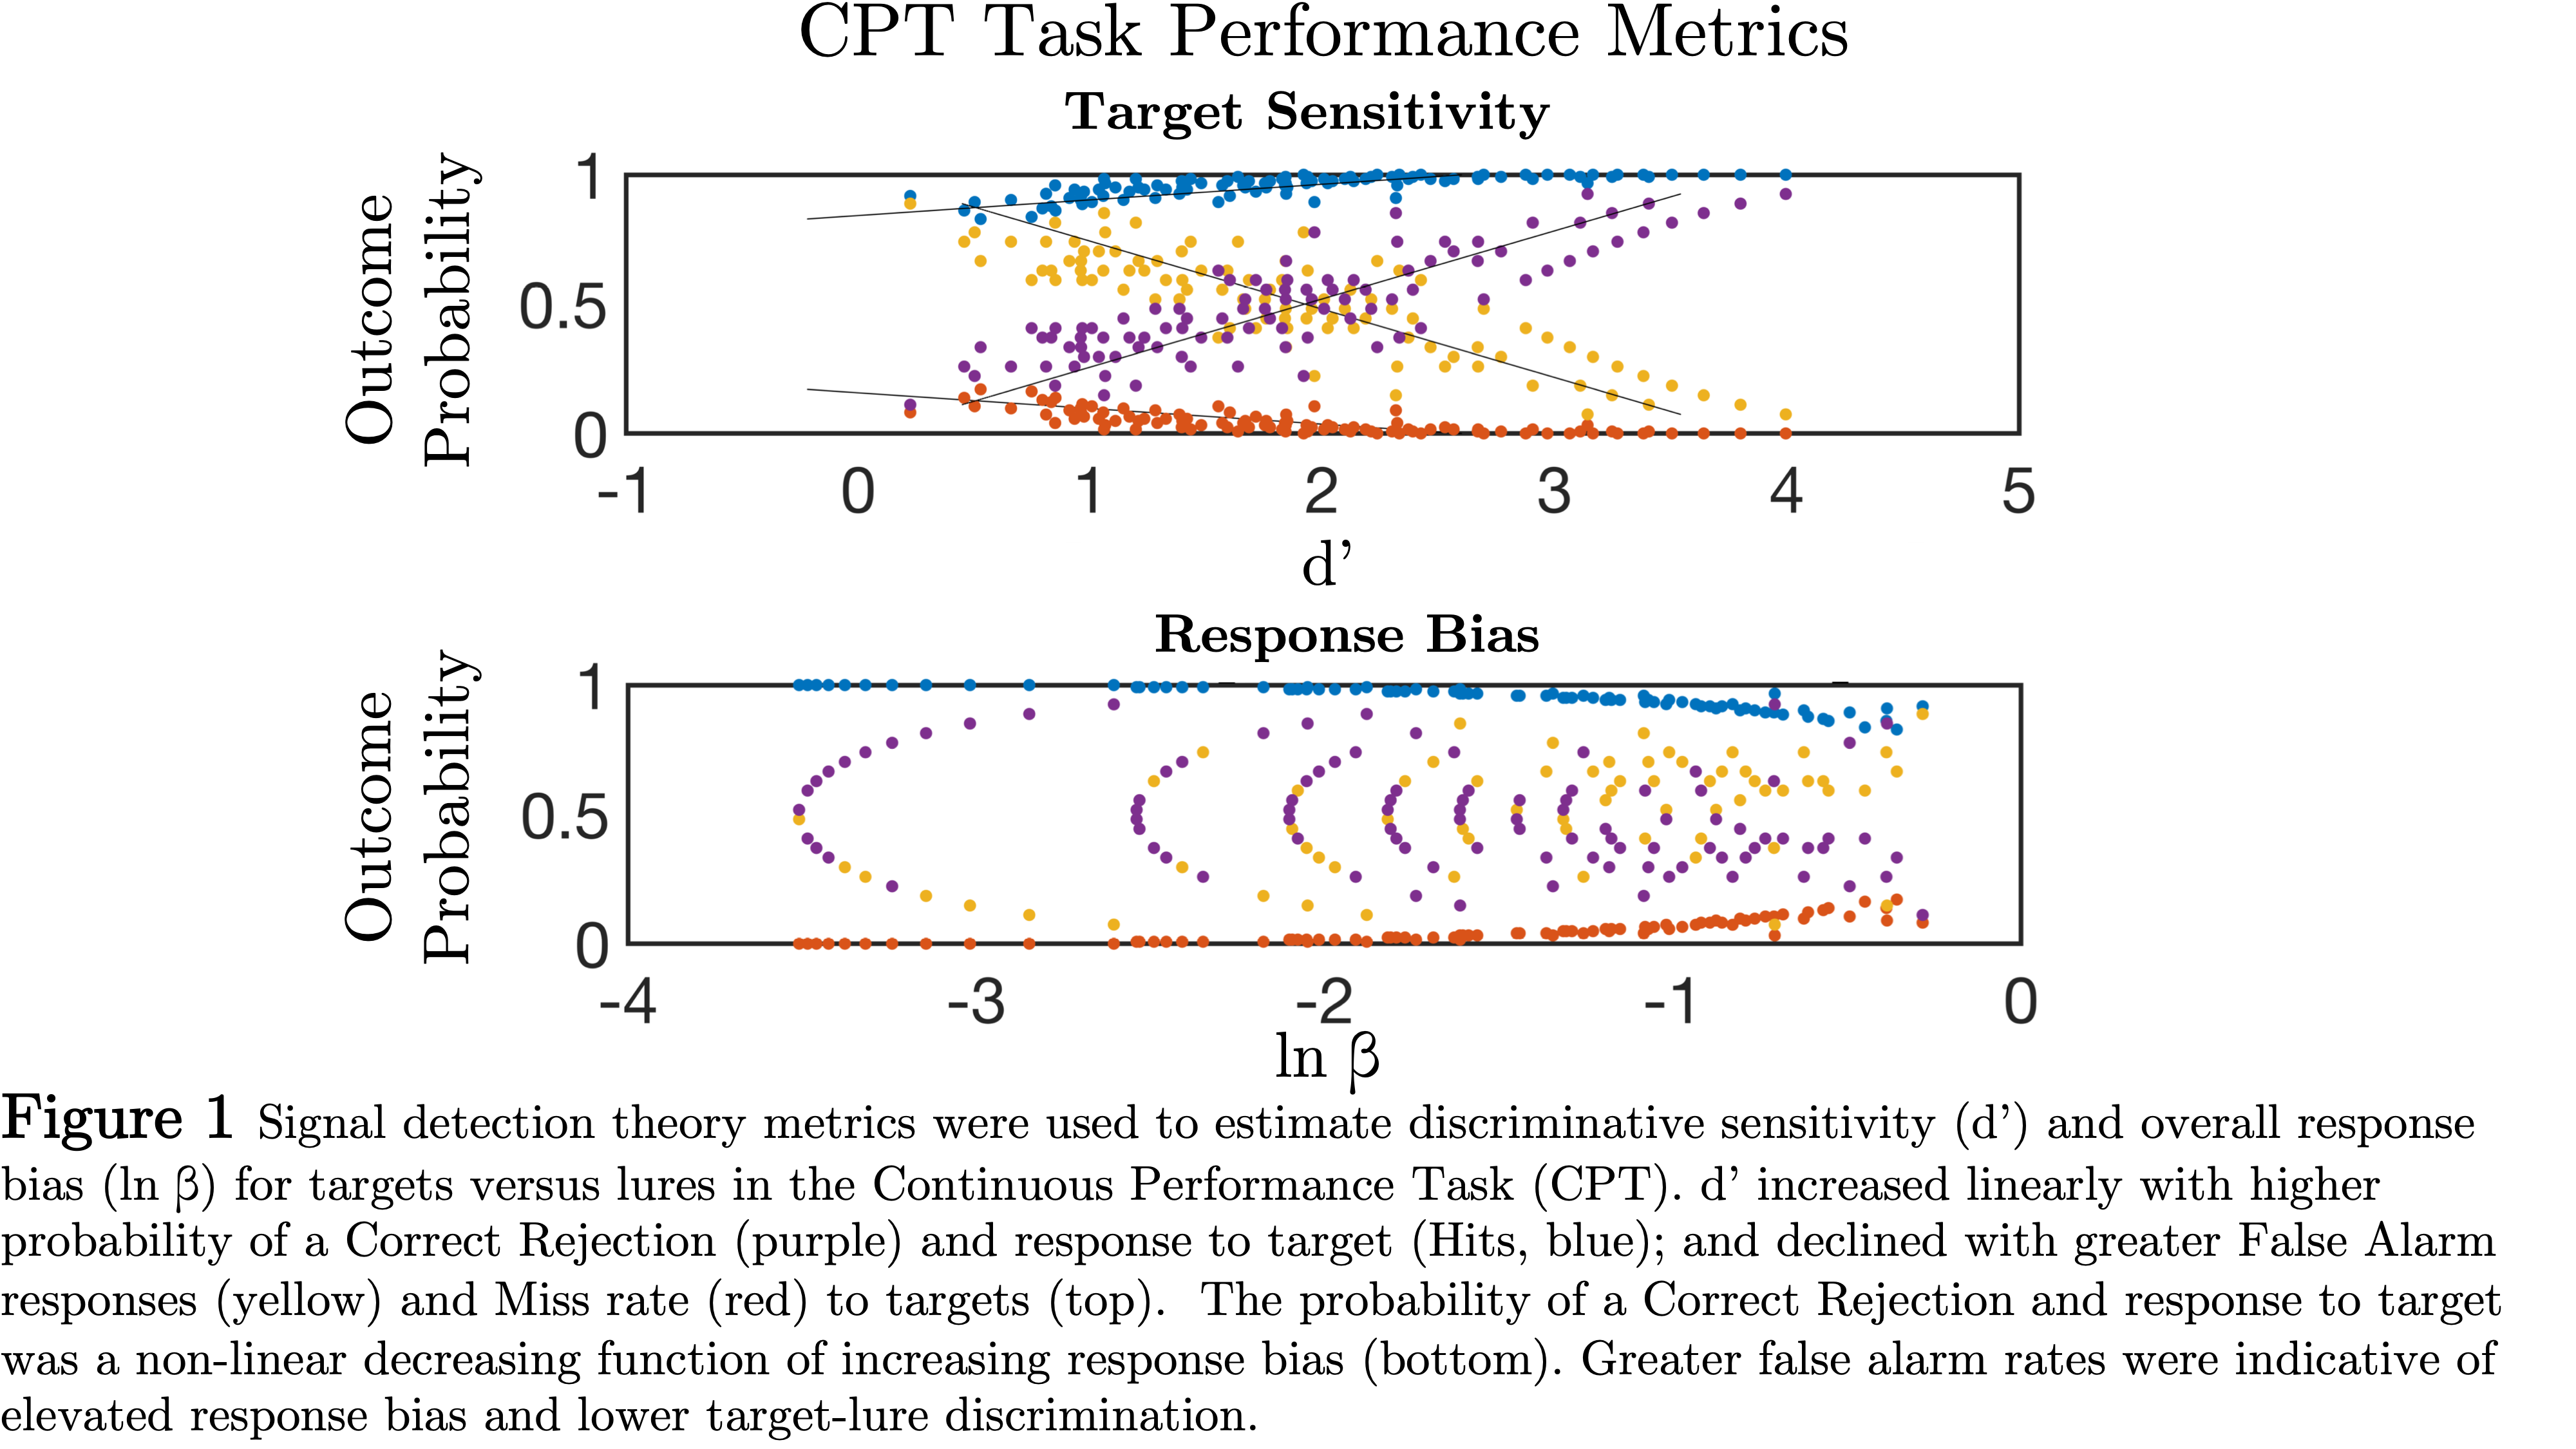
\includegraphics[width=\textwidth,height=\textheight,keepaspectratio]{Fig-1}
\caption{}
\label{fig:1}
\end{figure}

\begin{figure}[h!]
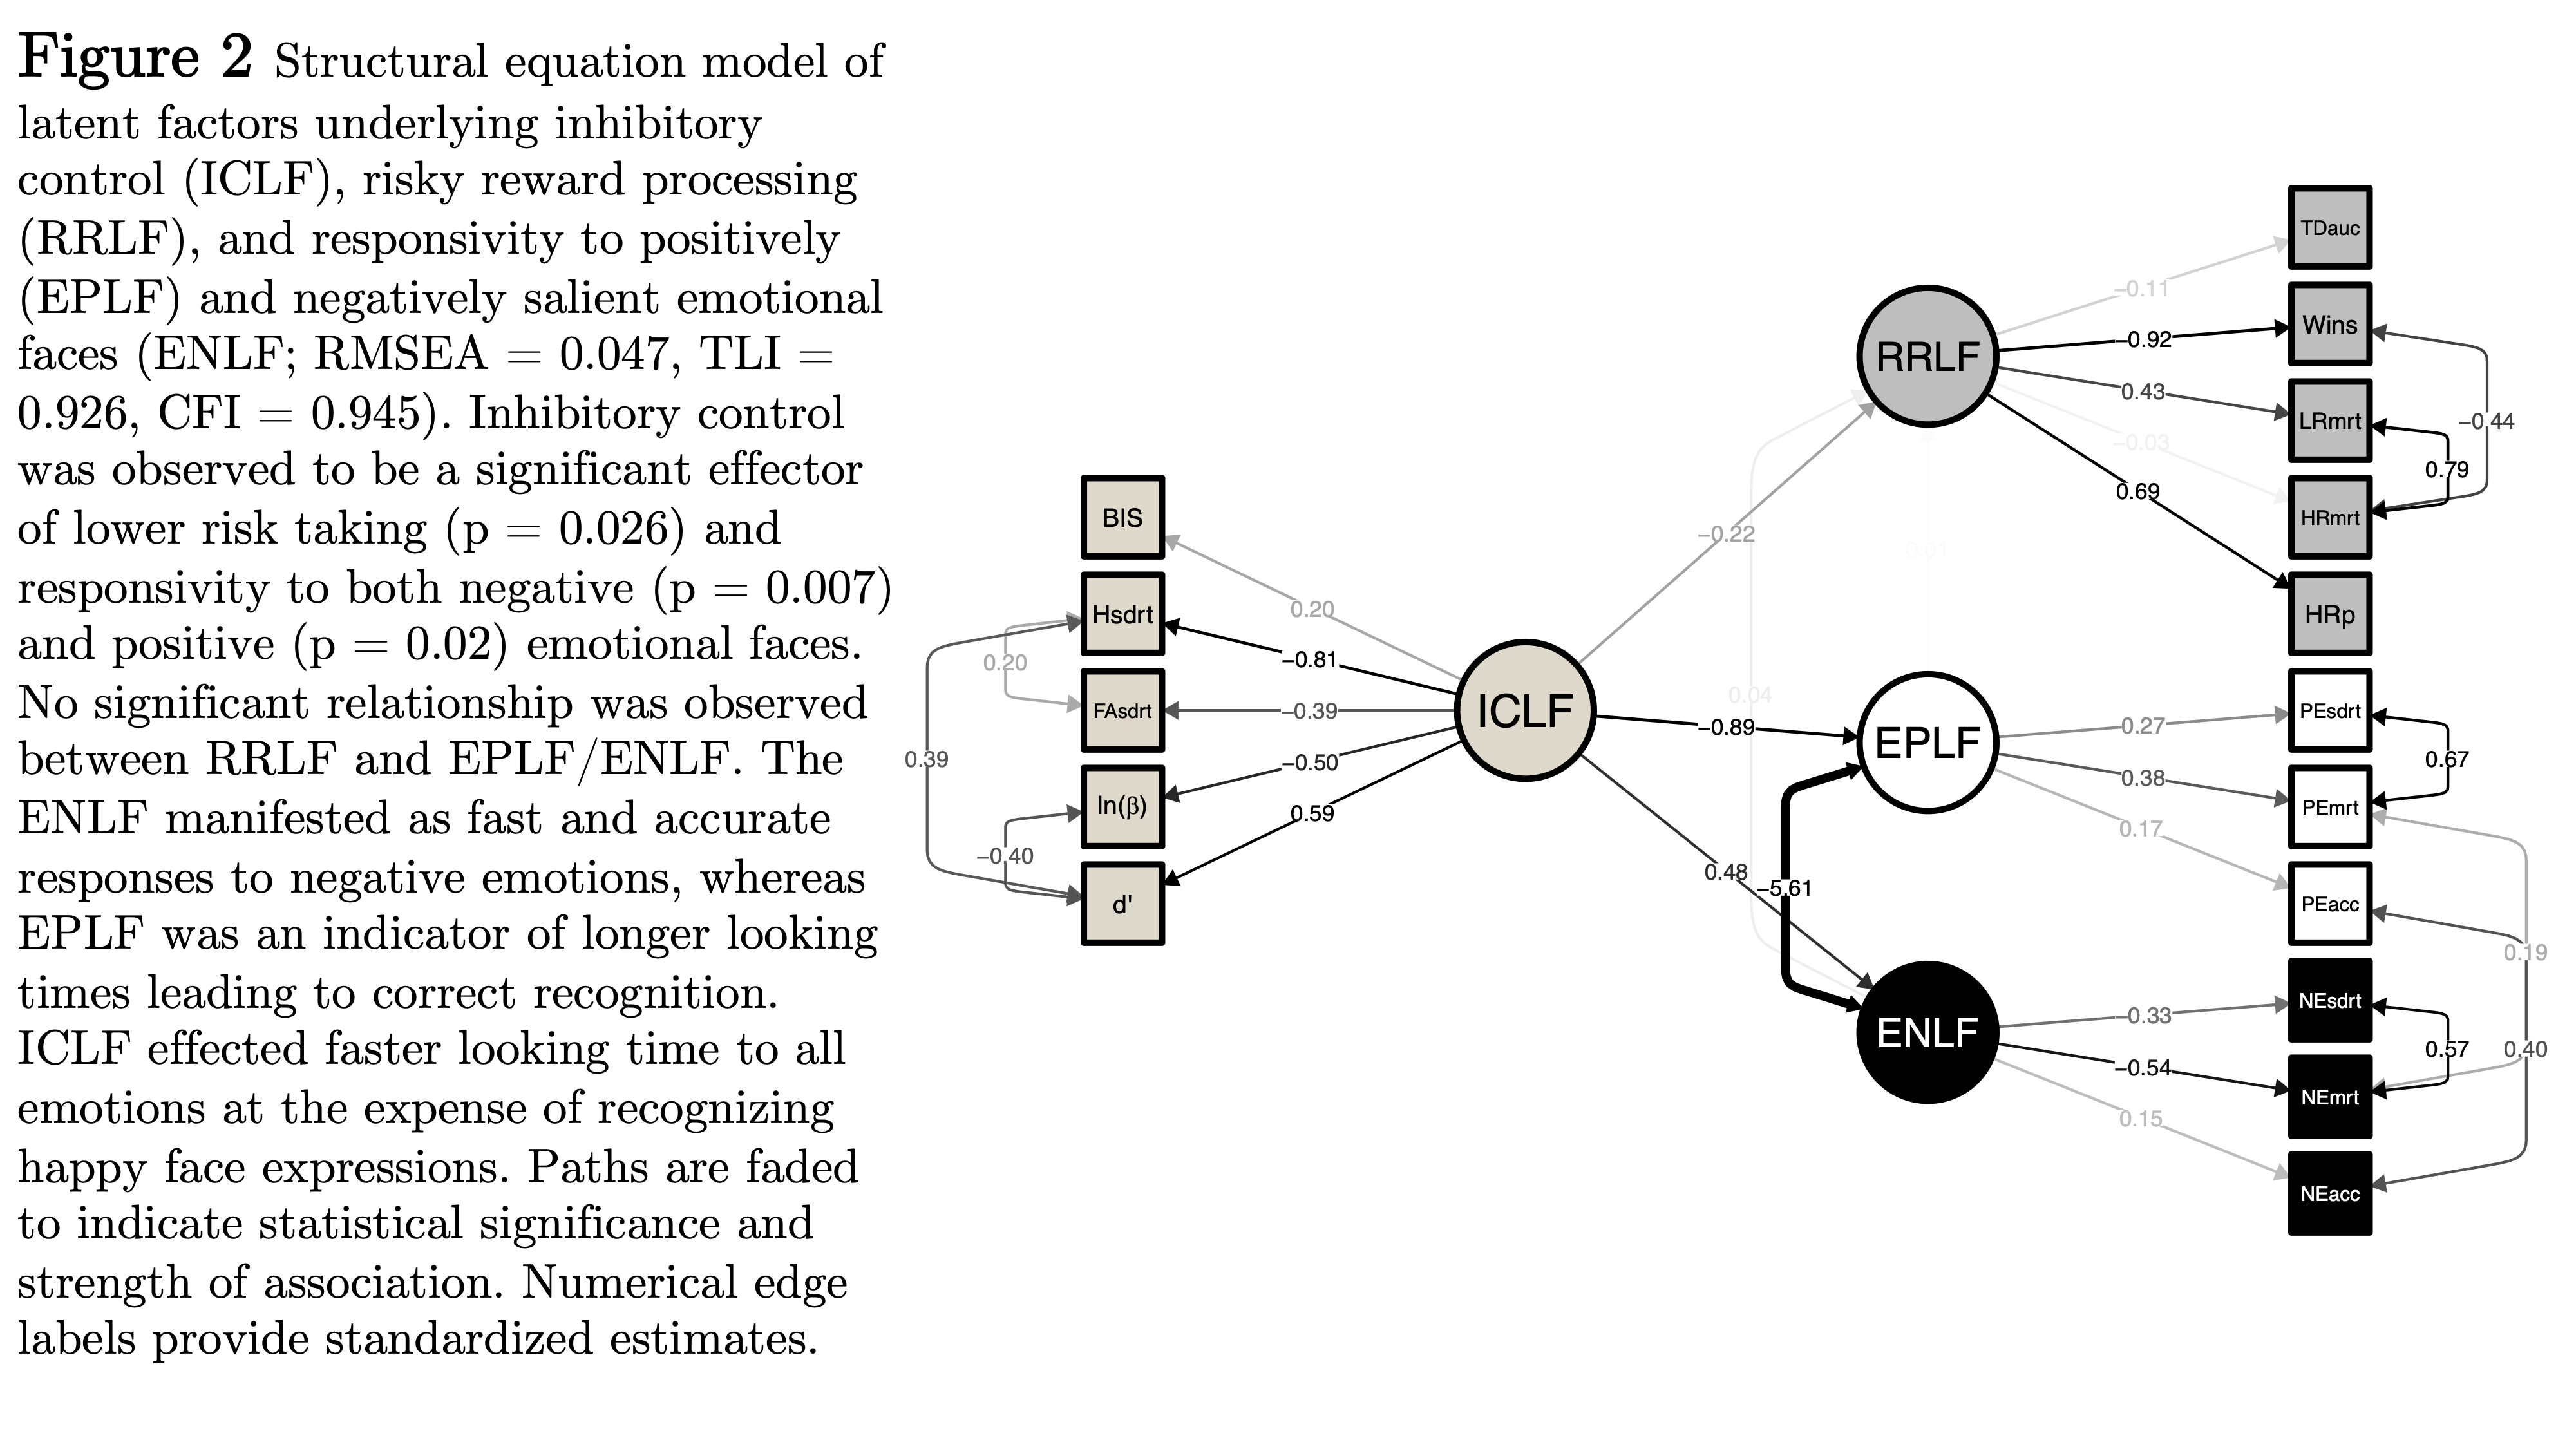
\includegraphics[width=\textwidth,height=\textheight,keepaspectratio]{Fig-2}
\label{fig:2}
\end{figure}

\begin{figure}[h!]
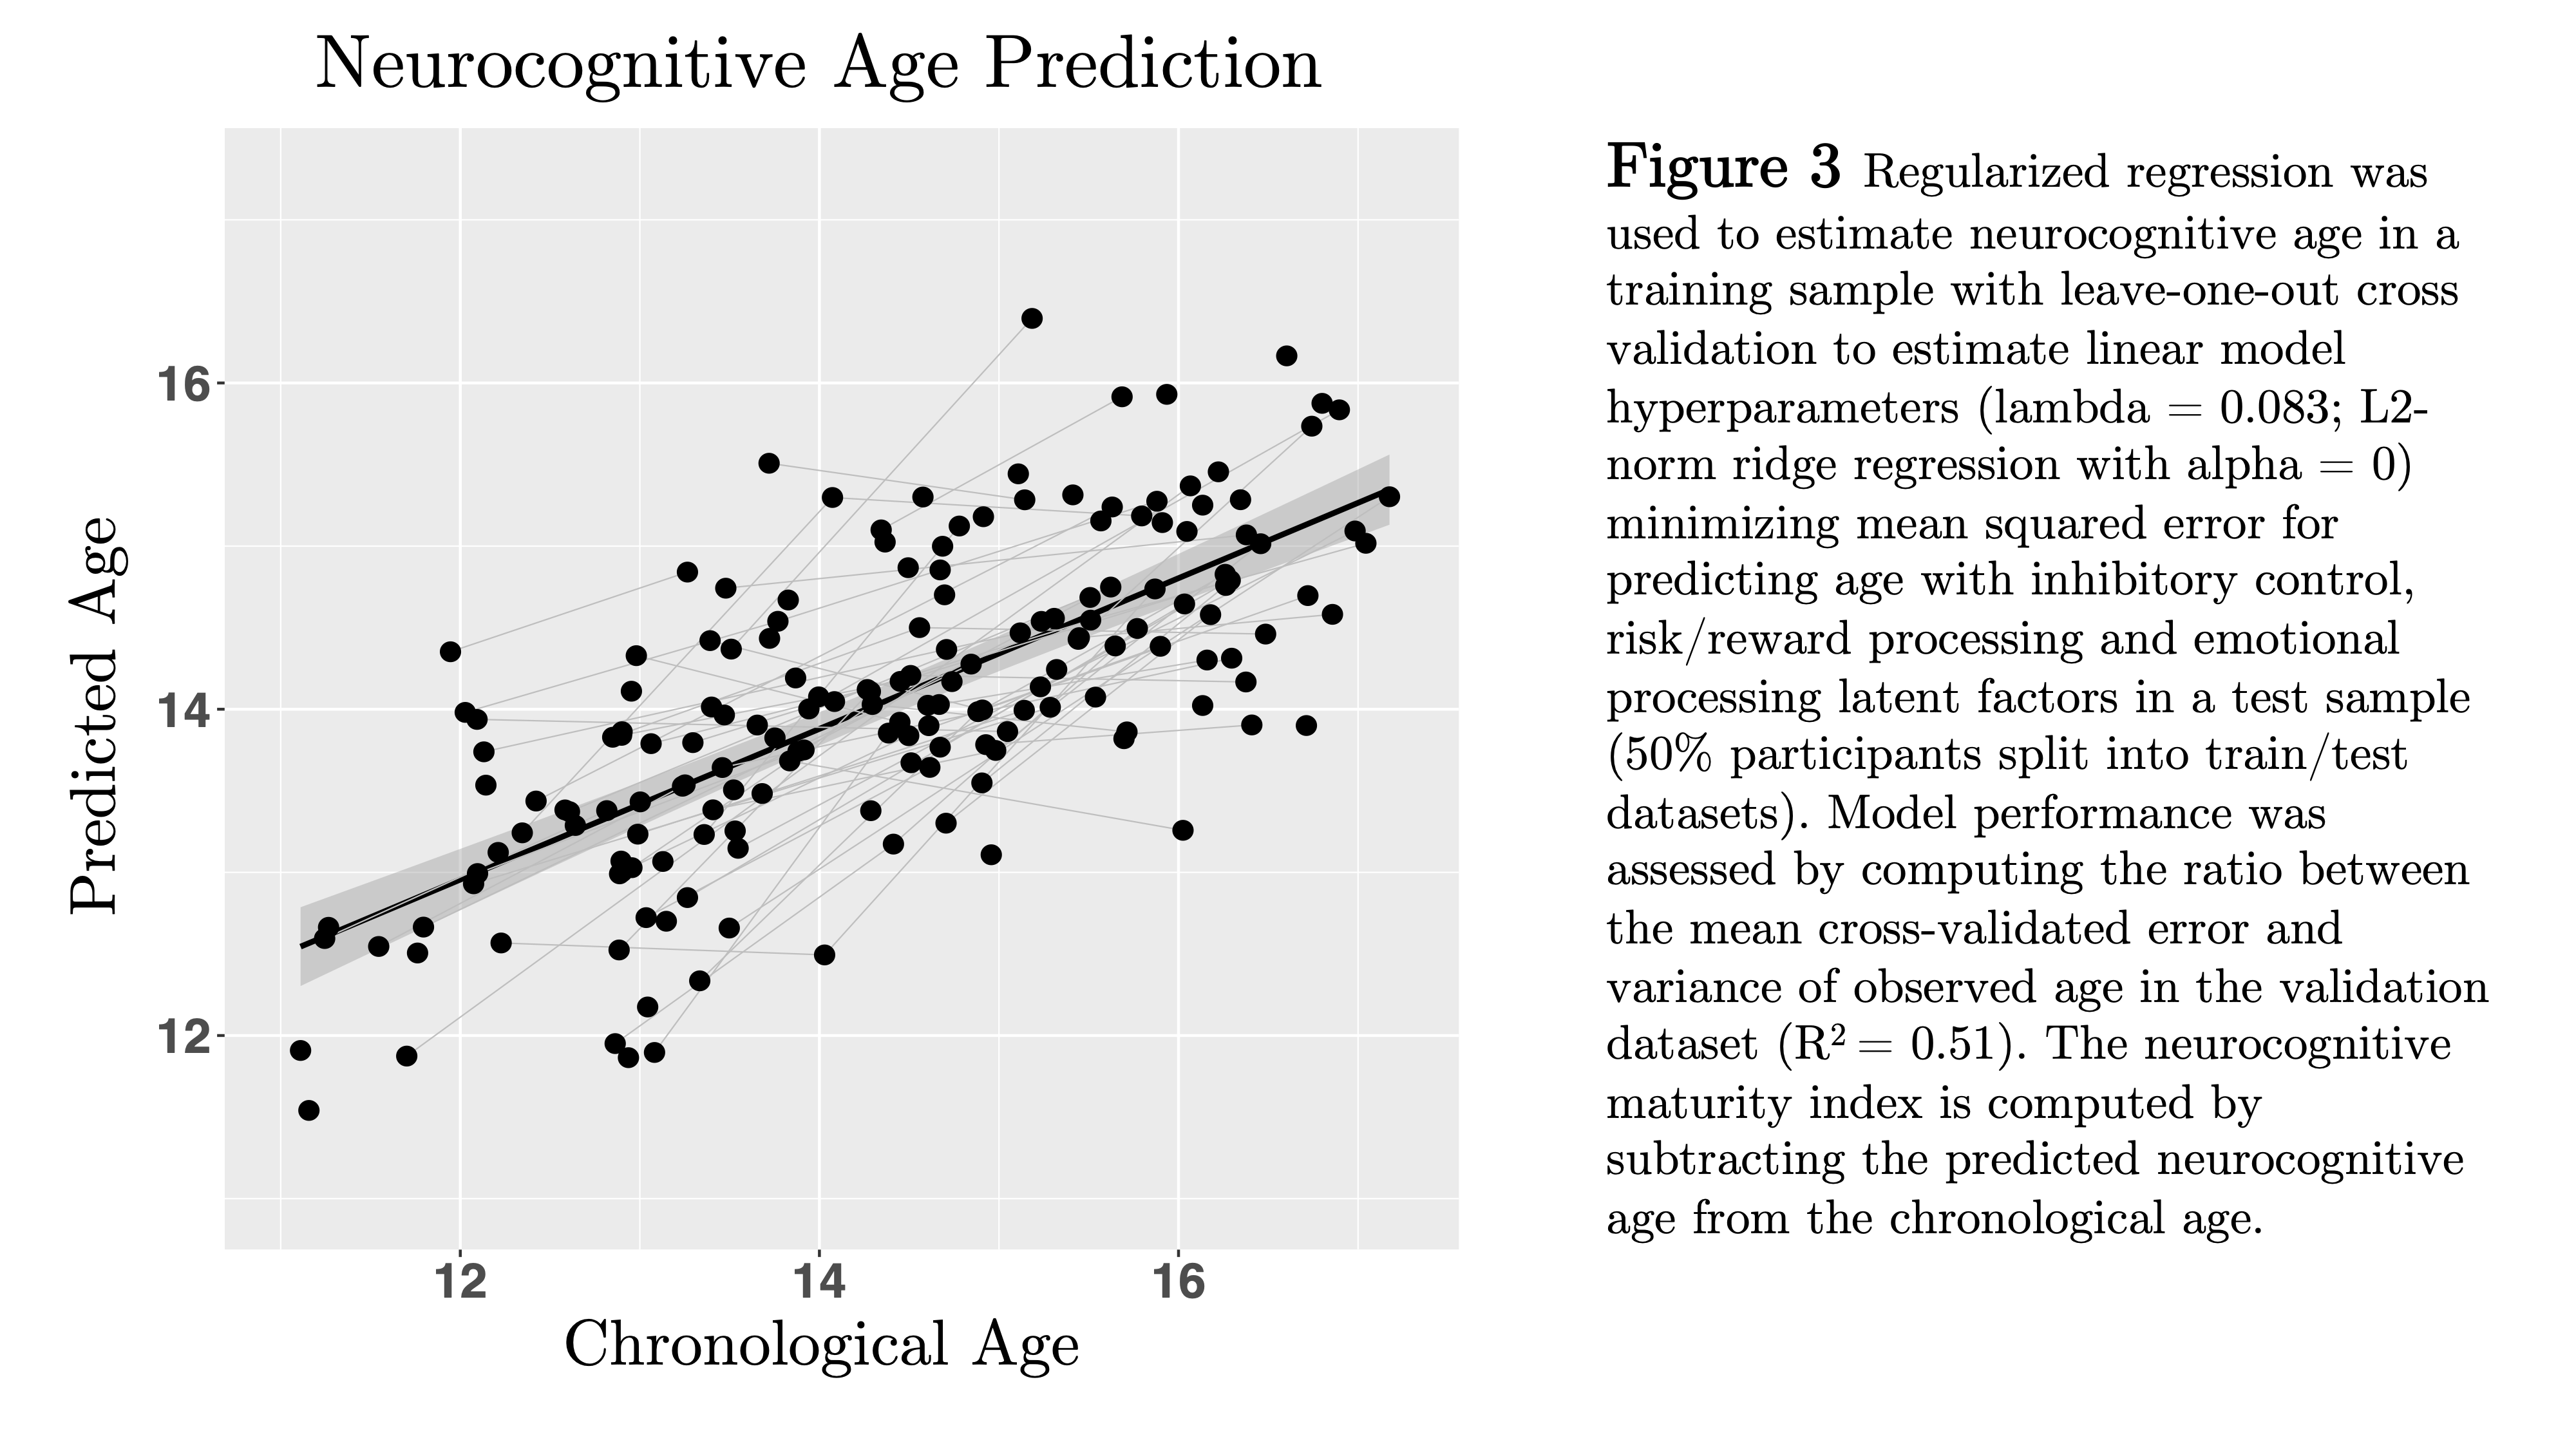
\includegraphics[width=\textwidth,height=\textheight,keepaspectratio]{Fig-3}
\label{fig:3}
\end{figure}

\begin{figure}[h!]
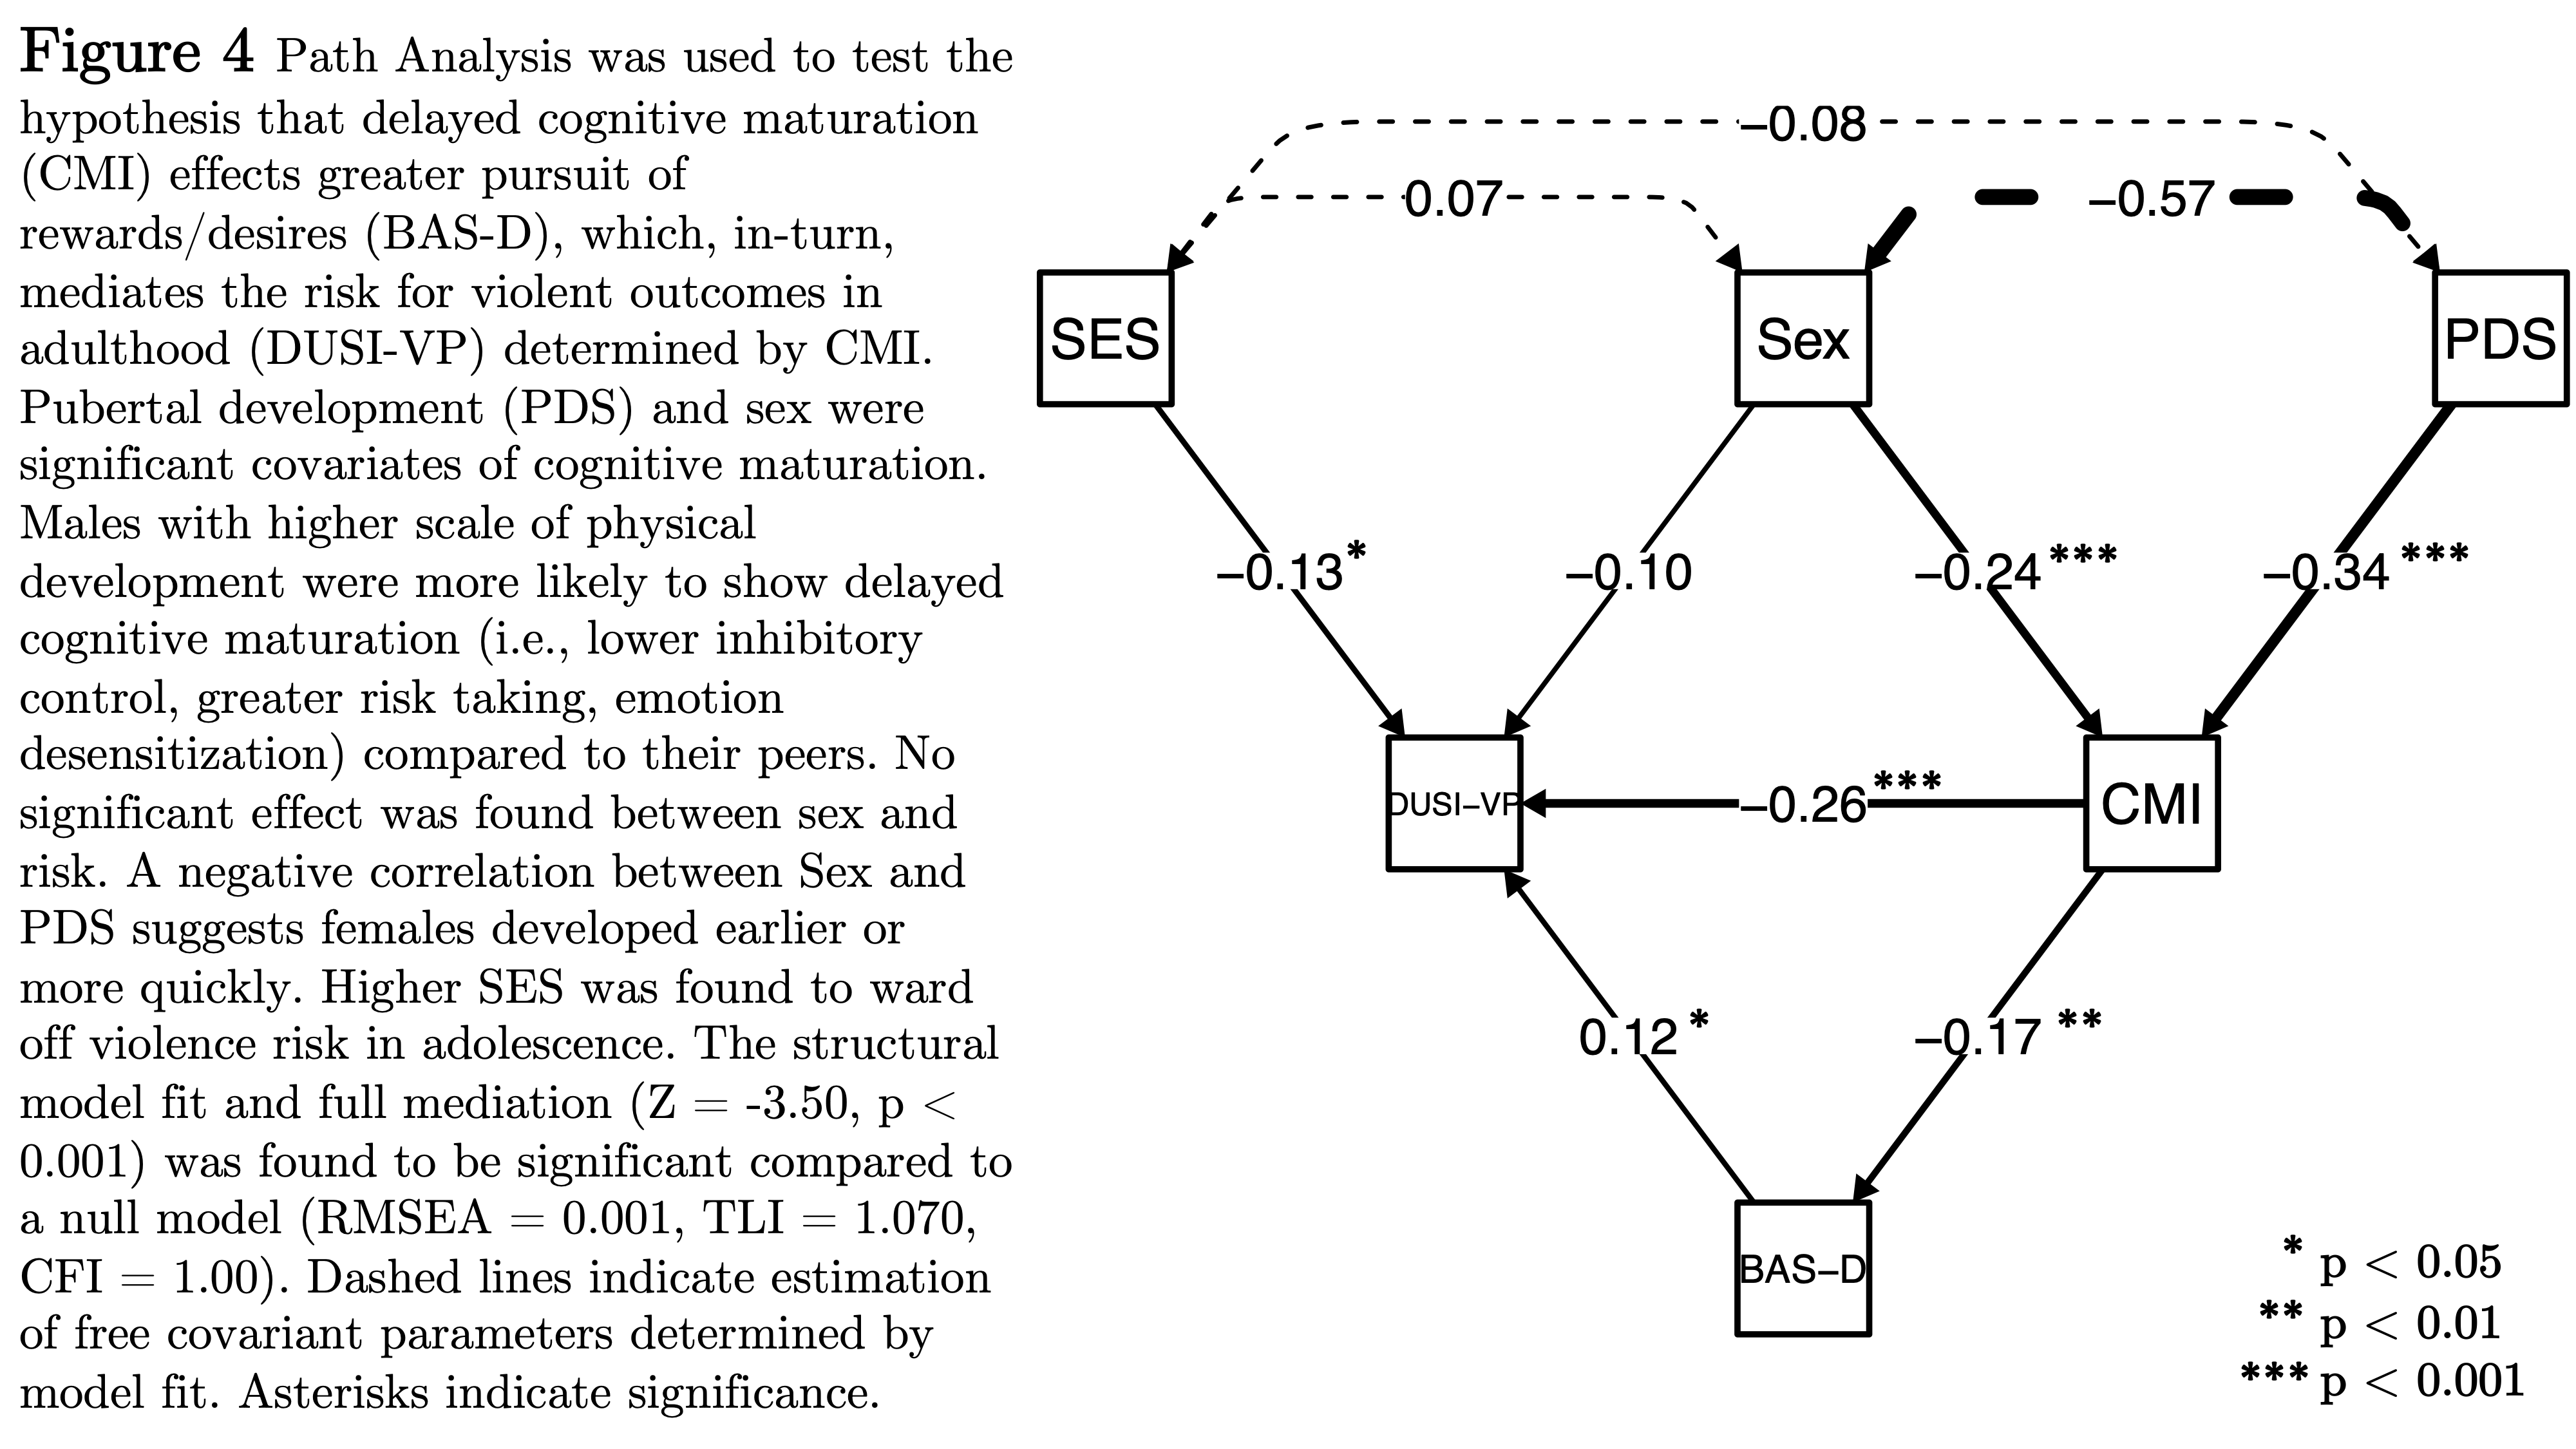
\includegraphics[width=\textwidth,height=\textheight,keepaspectratio]{Fig-4}
\label{fig:4}
\end{figure}

\begin{figure}[h!]
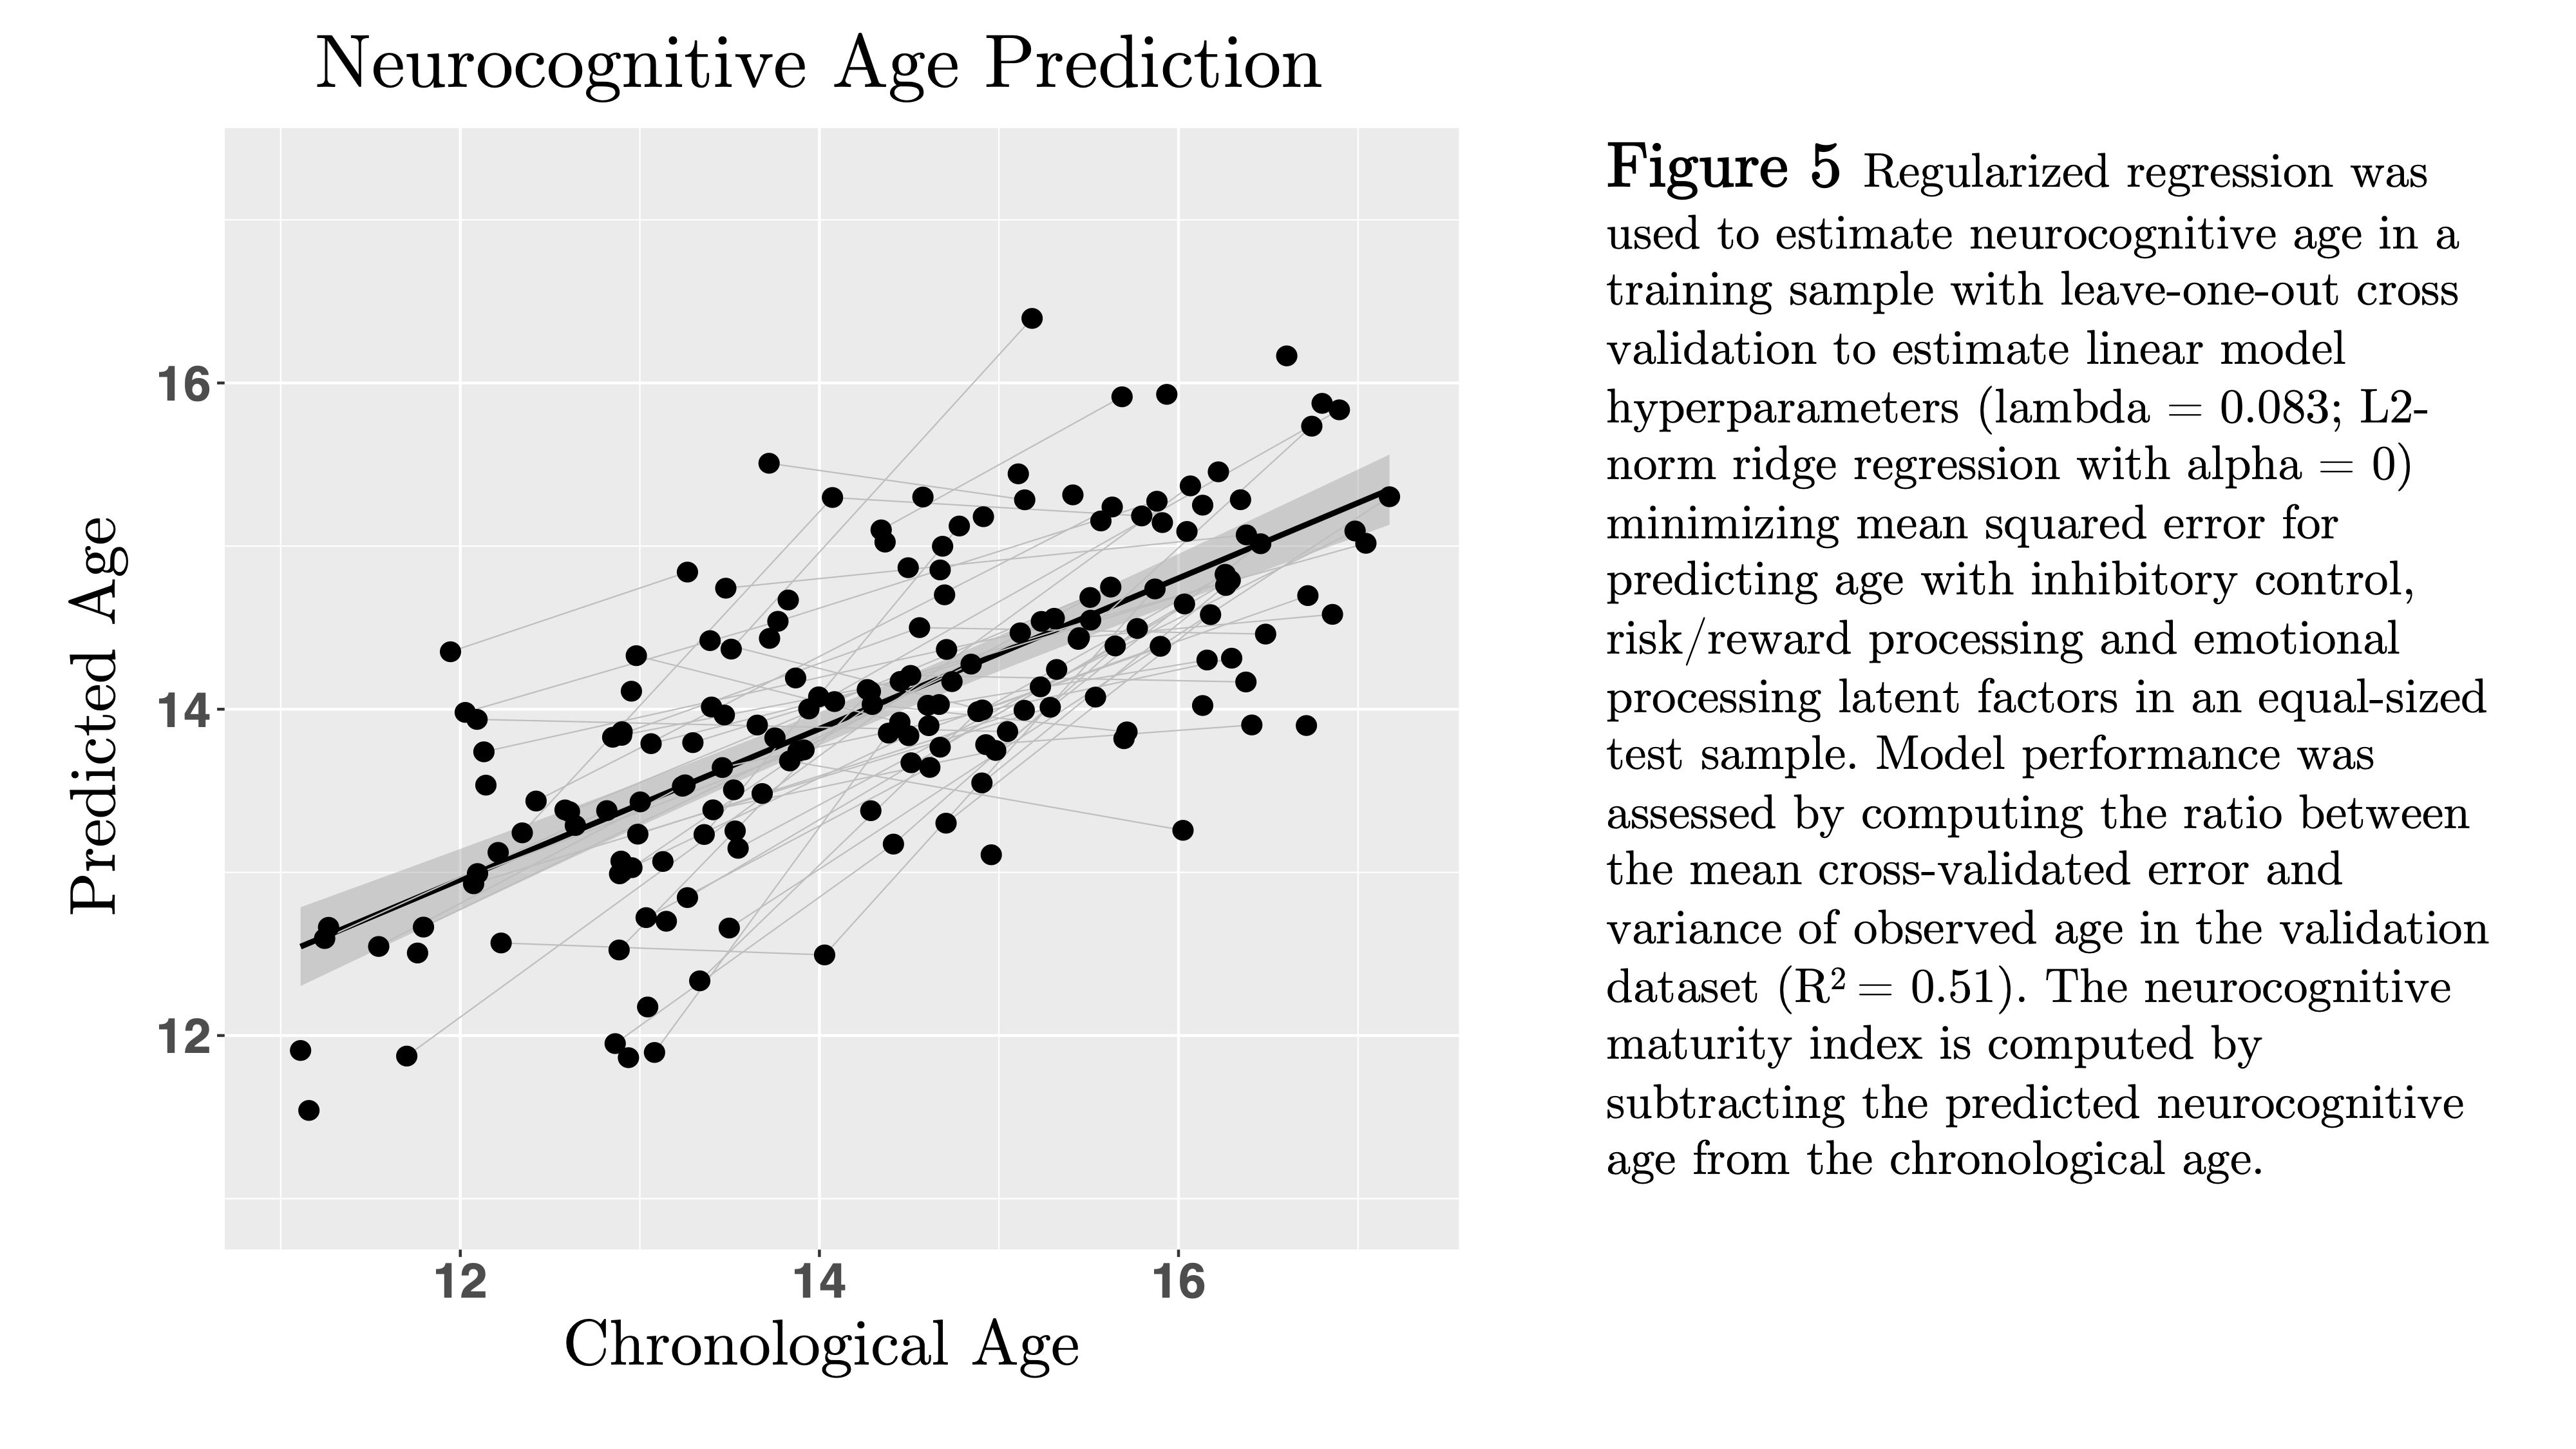
\includegraphics[width=\textwidth,height=\textheight,keepaspectratio]{Fig-5}
\label{fig:5}
\end{figure}

\begin{figure}[h!]
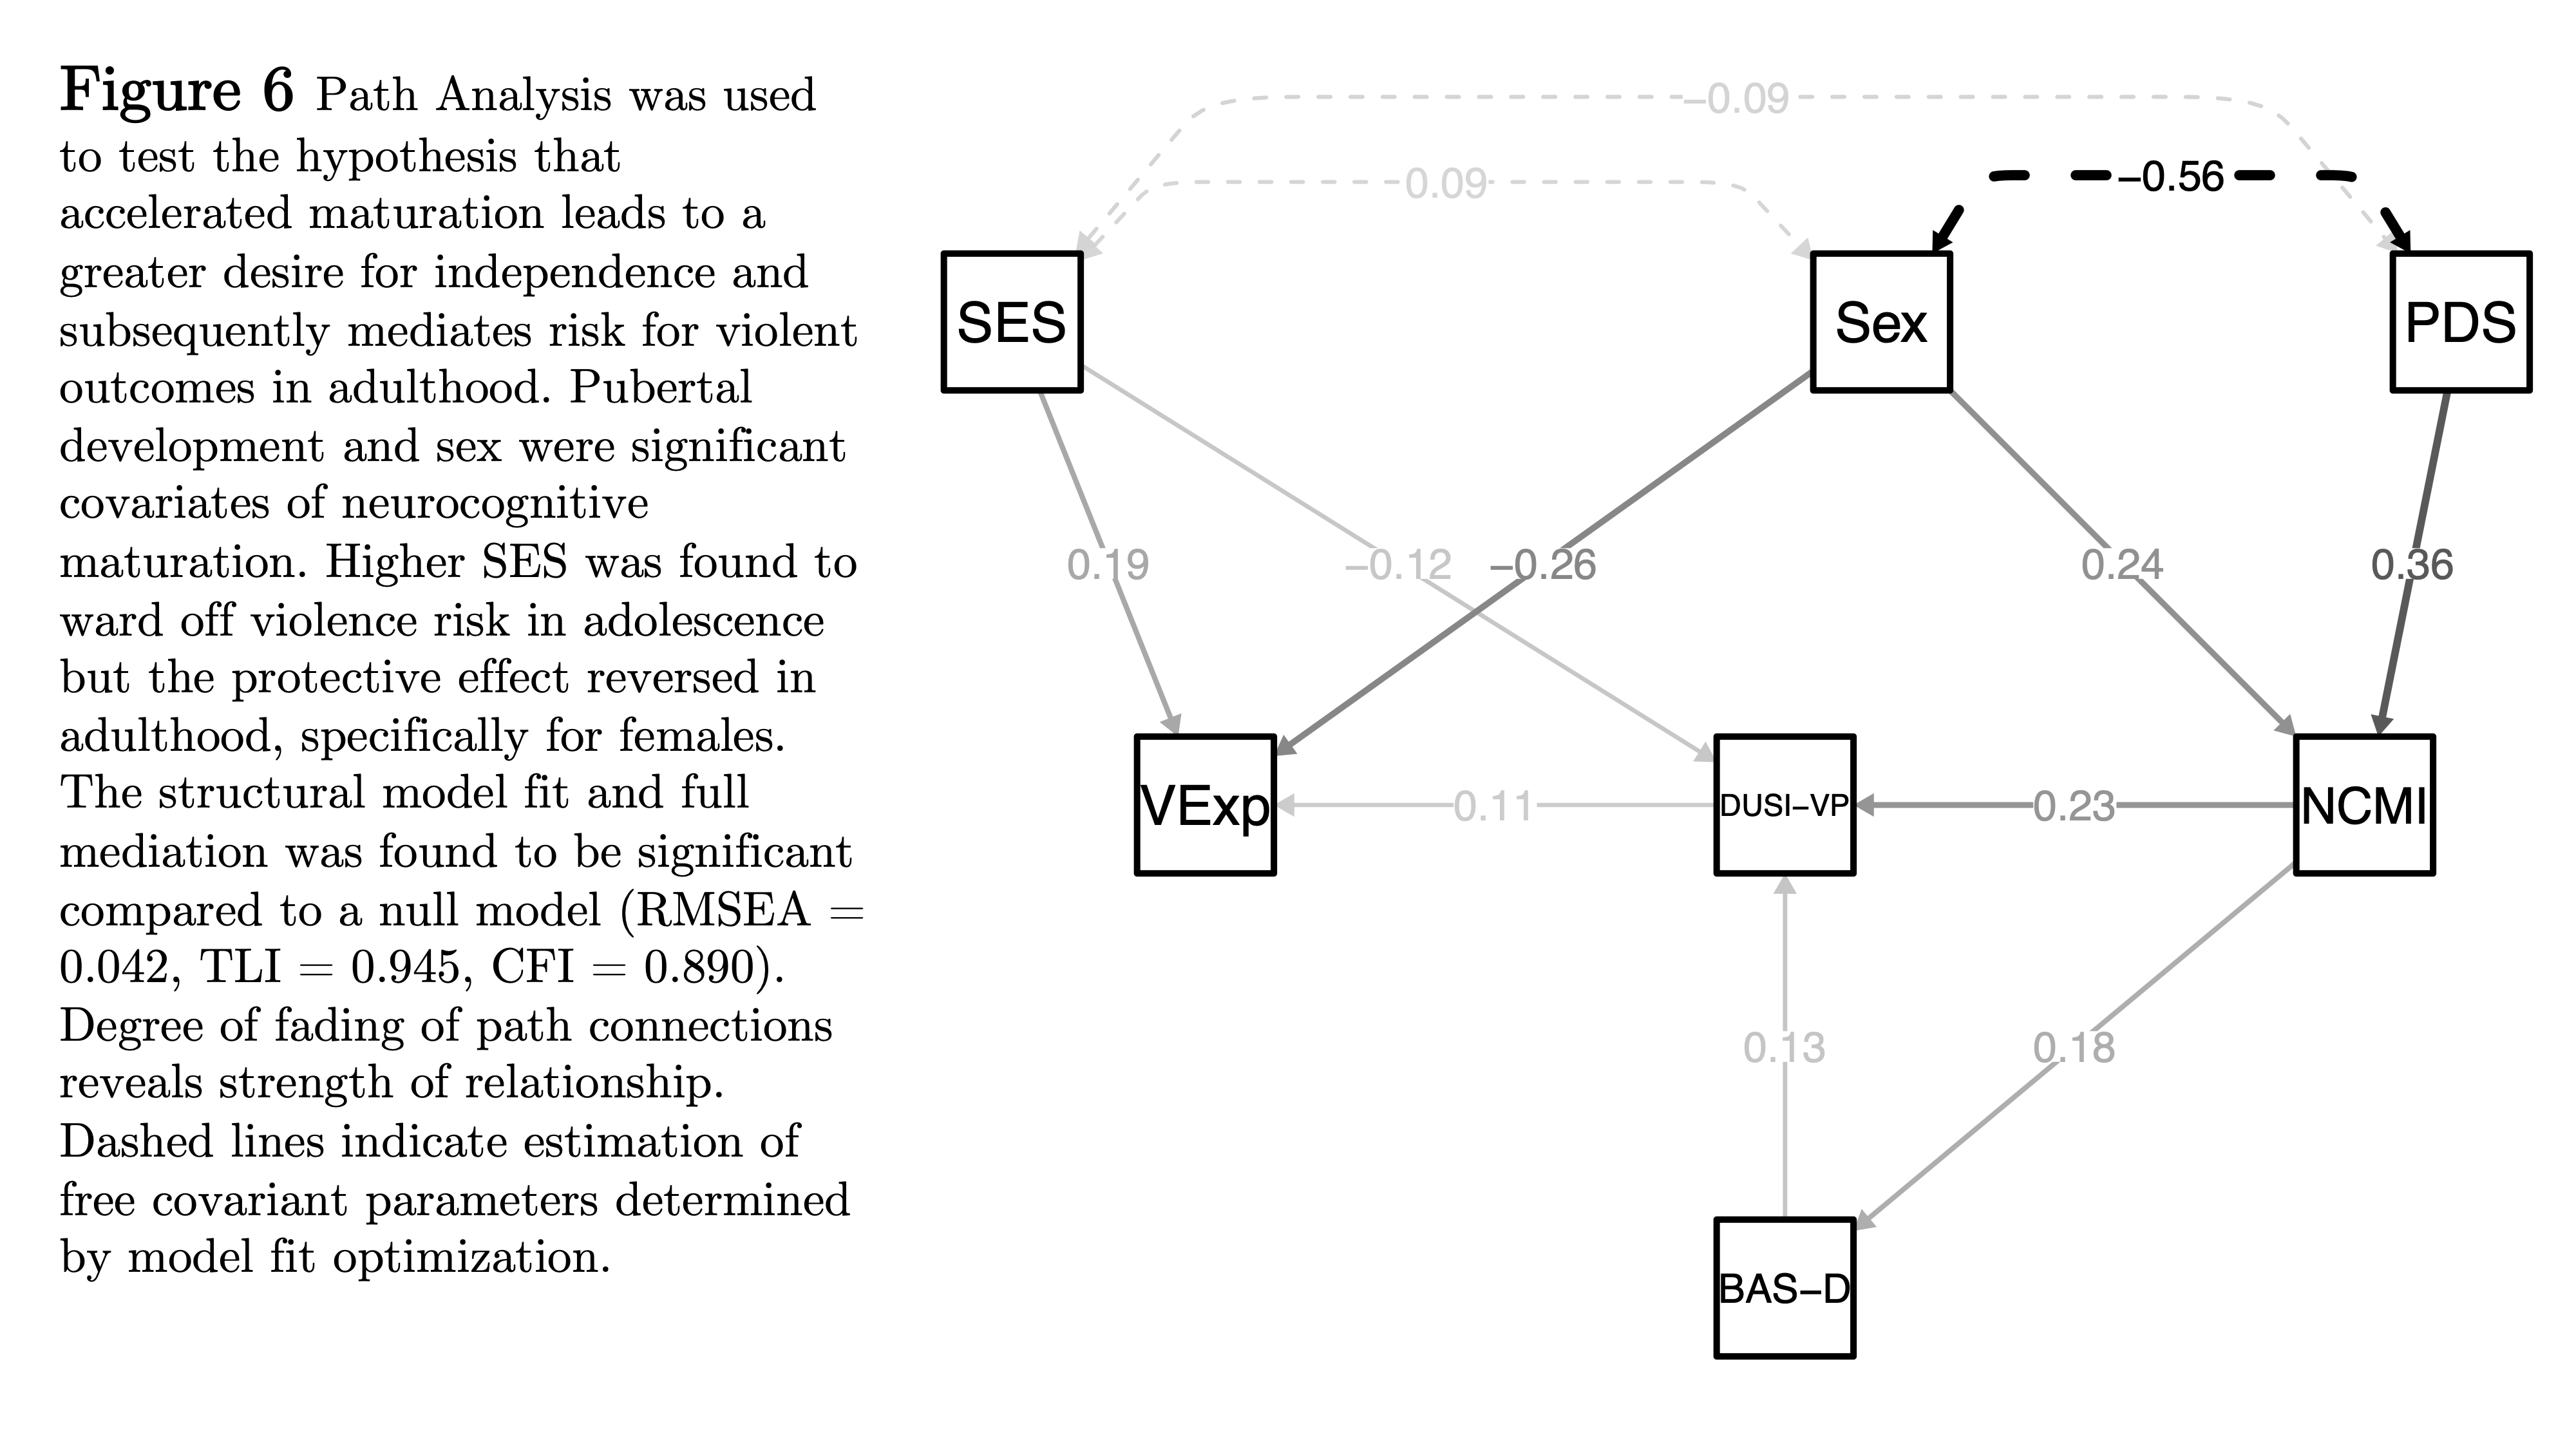
\includegraphics[width=\textwidth,height=\textheight,keepaspectratio]{Fig-6}
\label{fig:6}
\end{figure}

\newpage
\subsection{Tables}
\newpage
%\begin{table}[]

%Tables should be inserted at the end of the manuscript. Please build your table directly in LaTeX.Tables provided as jpeg/tiff files will not be accepted. Please note that very large tables (covering several pages) cannot be included in the final PDF for reasons of space. These tables will be published as \href{http://home.frontiersin.org/about/author-guidelines#SupplementaryMaterial}{Supplementary Material} on the online article page at the time of acceptance. The author will be notified during the typesetting of the final article if this is the case. 

% SEM Latent Variables:
%                         Estimate  Std.Err  z-value  P(>|z|)
%   neg_emot =~                                              
%     efr_negativ_cc         0.133    0.073    1.821    0.069
%     efr_ngtv_mn_rt        -0.476    0.168   -2.839    0.005
%     efr_ngtv_sd_rt        -0.287    0.106   -2.709    0.007
%   pos_emot =~                                              
%     efr_happnss_cc         0.075    0.165    0.455    0.649
%     efr_hppnss_mnr         0.171    0.359    0.476    0.634
%     efr_hppnss_sd_         0.119    0.248    0.481    0.631
%   reward_proc =~                                           
%     wf_hr_dcsn_pr_         0.677    0.065   10.424    0.000
%     wf_hr_mn_rt_th        -0.028    0.082   -0.340    0.734
%     wf_lr_mn_rt_th         0.418    0.060    6.936    0.000
%     wf_cmltv_wnnn_        -0.896    0.071  -12.706    0.000
%     tmprl_dscntng_        -0.103    0.060   -1.713    0.087
%   inhibitory_control =~                                    
%     gonogo.dprime          0.588    0.107    5.479    0.000
%     gonogo.beta           -0.588    0.140   -4.185    0.000
%     gng.Incrrc.G..        -0.388    0.093   -4.186    0.000
%     gng.Crrct.G.r.        -0.806    0.128   -6.289    0.000
%     bis                    0.202    0.066    3.055    0.002




\bibliography{eldamaty_ncmi_2020b}

\bibliographystyle{frontiersinSCNS_ENG_HUMS}

%%% Make sure to upload the bib file along with the tex file and PDF
%%% Please see the test.bib file for some examples of references

\end{document}
